%% LyX 2.2.0 created this file.  For more info, see http://www.lyx.org/.
%% Do not edit unless you really know what you are doing.
\documentclass[12pt,english]{kuthesis}
\usepackage{mathptmx}
\usepackage{MnSymbol}
\renewcommand{\sfdefault}{lmss}
\renewcommand{\ttdefault}{lmtt}
\usepackage[T1]{fontenc}
\usepackage[utf8]{inputenc}
\usepackage{geometry}
\geometry{verbose,tmargin=1in,bmargin=1in,lmargin=1in,rmargin=1in}
\setcounter{secnumdepth}{3}
\setcounter{tocdepth}{3}

\usepackage{xcolor}
\usepackage{babel}
\usepackage{url}
\usepackage{graphicx}
\usepackage{setspace}
\usepackage{esint}
\usepackage[authoryear]{natbib}

\usepackage{bussproofs}
\usepackage{semantic}
\usepackage{framed}
\usepackage{minted}
\usepackage{cmll}
\usepackage{amsthm}
\usepackage{pdflscape}
\usepackage{tikz-qtree}
\usepackage{stmaryrd}

\renewcommand\qedsymbol{$\blacksquare$}

\newtheorem{theorem}{Theorem}

\doublespacing
\usepackage[unicode=true,
 bookmarks=true,bookmarksnumbered=false,bookmarksopen=false,
 breaklinks=true,pdfborder={0 0 0},pdfborderstyle={},backref=false,colorlinks=true]
 {hyperref}
\hypersetup{pdftitle={University of Kansas Thesis Template},
 pdfauthor={Apoorv Ingle},
 pdfsubject={A Thesis},
 urlcolor={blue},citecolor={blue},allcolors={blue}}
\usepackage{cleveref}
\crefformat{section}{\S#2#1#3} % see manual of cleveref, section 8.2.1
\crefformat{subsection}{\S#2#1#3}
\crefformat{subsubsection}{\S#2#1#3}

\makeatletter

%%%%%%%%%%%%%%%%%%%%%%%%%%%%%% LyX specific LaTeX commands.
\providecommand{\LyX}{\texorpdfstring%
  {L\kern-.1667em\lower.25em\hbox{Y}\kern-.125emX\@}
  {LyX}}
%% Because html converters don't know tabularnewline
\providecommand{\tabularnewline}{\\}
%%%%%%%%%%%%%%%%%%%%%%%%%%%%%% User specified LaTeX commands.
\newcommand{\BI}{\textbf{\em BI}}
\newcommand\sepimp{\mathrel{-\mkern-6mu*}}

\newcommand{\M}{\mathcal{M}}
\newcommand{\Unf}{\mathcal{U}}

\newcommand{\SeFun}[1]{\texttt{SeFun}\ #1}
\newcommand{\ShFun}[1]{\texttt{ShFun}\ #1}
\newcommand{\Un}[1]{\texttt{Un}\ #1}
\newcommand{\Let}[3]{\texttt{let}\ #1 = #2\ \texttt{in}\ #3}
\newcommand{\Case}[2]{\texttt{case}\ #1\ \texttt{of}\ #2}
\newcommand{\CaseSh}[2]{\texttt{case}_{sh}\ #1\ \texttt{of}\ #2}
\newcommand{\CaseSe}[2]{\texttt{case}_{se}\ #1\ \texttt{of}\ #2}
\newcommand{\Pair}[1]{\langle #1 \rangle}
\newcommand{\TODO}[1]{{\begin{framed}{\color{red} #1}\end{framed}}}
\newcommand{\HaskellF}[1]{\mintinline{haskell}{#1}}
\newcommand{\qub}{QuB}

% used to align decimals in tables according to APA style
\usepackage{dcolumn}
\usepackage{booktabs}

% Set the title and author info
\title{\qub : A Resource Aware Functional Language}
\author{Apoorv Ingle}


\dept{Electrical Engineering and Computer Science}
\degreetitle{Master of Science}
\papertype{Thesis} %or Thesis (Whatever you put will appear on p.2)
%% It is vital to have 7 entries, even if some are empty for committee and role
%% I mean, it is vital to leave the empty place holders
\committee{Dr. J. Garrett Morris}{Dr. Perry Alexandar}{Dr. Andy Gill}{Dr. Prasad Kulkarni}{}{}{}
\role{Chairperson}{}{}{}{}{}{}
%AT Most 7 members allowed, last here is blank on purpose to demonstrate
%flexibility

%% The following is OPTIONAL. Remove all 3 of the next 3 lines
%% to leave dates blank. If dates are included, then both dates
%% must be included.
\@printd@testrue
\datedefended{July 21, 2018}
\dateapproved{July 21, 2018}

%% These settings are now in the kuthesis.cls file, but users are free
% to customize. listings has great documentation online
%% When listings are used, break lines
%\lstset{
 %    breaklines=true,  % sets automatic line breaking
 %    breakindent=2em,
 %    breakatwhitespace=true,  % sets if automatic breaks should
 %   breakautoindent=true
%}

\@ifundefined{showcaptionsetup}{}{%
 \PassOptionsToPackage{caption=false}{subfig}}
\usepackage{subfig}
\makeatother

\usepackage{listings}
\renewcommand{\lstlistingname}{\inputencoding{latin9}Listing}

\begin{document}
\begin{romanpages}

\maketitle
\begin{abstract}
  Modern programming languages treat resources as normal values.
  They have different semantics at runtime that does not match with its static
  semantics. For example, file handles or database connections are treated as integers
  in C. Modern functional programming languages like Haskell try to improve this
  by wrapping them in IO monads. While it is an improvement over imperative languages,
  well typed programs may have runtime errors. Type systems based on linear logic[\cite{girard_linear_1987}]
  promise a way to introduce the efficient resource handling in programs.
  %There have been numerous attempts to make use of linear logic in programming languages.
  %It has made its way into some parts of programming languages
  %such as garbage collectors and also type systems (Rust and Clean).
  While the these is more expressive than intuistionistic logic, there are various practical issues
  that prohibit leveraging it to its fullest degree in programming languages.
  In this thesis, we take a different view over the resource management problem by concentrating
  on sharing or separation of resources which been studied in a theoritical
  setting as the logic of bunched implications (\BI)[\cite{ohearn_logic_1999}].

  We design and implement \qub\, a prototype language that is Curry-Howard interpretation of the logic
  of \BI\ [\cite{ohearn_bunched_2003}]---$\alpha\lambda$-calculus---by introducing 2 new type
  constructors of arrow type: sharing arrow ($\rightarrow$) and separating arrow($\sepimp$) to replace
  the usual notion of function arrows of simply typed lambda calculus. Sharing arrows imply that functions
  share resources with its arguments, while separating arrows imply that functions do not share resources with its arguments.
  We base our work on Quill [\cite{morris_best_2016}] which express linear types in a functional language.
  We realize that the interaction of unrestricted types and sharing and separating is harmless as program entities that
  do not have a sense of resourcefulness can be duplicated or dropped anytime without
  any adverse implications and all existing programs typecheck.
  % haivng unrestricted types
  % are realizations of existing purely functional programs.

  % Complexity of software systems has been increasing forever. Automation of tasks
  % provides consistency, correctness and speed at a much greater degree than humans.
  % complex software systems find their use in various fields ranging from automobiles, aircrafts,
  % financial institutions and even medicine. Higher level programming languages
  % are used to program these software systems and developing them requires
  % adequate understanding of the programming language along with problem domain.
  % Structured programming techniques ensures maintanability and extensibility
  % of the software application. Types and functional programming style helps maintain
  % structure by making it possible to run algorithmic checks to ensure sanity.
  % I have no idea what I am talking about. TODO! get back on track

  %  What is quil?
  % Quill is a purely functional language that uses
  % qualified types and a varient of linear logic to keep track of resources.
  % We introduce a new type class to express unrestrictedness
  % of a type, define the degree of unrestrictedness of classes
  % and a concept of sharing or separation of closures for functions

  % What am I trying to doing here?
  % Make Quill work. Write programs in them and check and see
  % how painful it is.
  % We realize that we have 2 kinds of pairs, a sharing pair and a separating pair depending
  % on the arrow we use. We try to formalize other structures such as Lists, non-empty lists
  % datatypes (recursive and non-recursive) and type classes such as functor, applicative and
  % monads with specific instances of each.

\begin{acknowledgementslong}
%%if you want a "quote" environment for acknowledgements,
%% use acknowledgements instead of acknowledgementslong
  TODO TODO TODO DO DO DO DO.
% I would like to thank all of the little people who made this thesis
% possible. Sleepy, Dopey, Grumpy, you know who you are.

\end{acknowledgementslong}
\end{abstract}
\tableofcontents{}

\listoffigures

\listoftables

\end{romanpages}

\chapter{Background Work}
% TODO should change title

\section{Type Inference Algorithm}
Algorithm $\mathcal{W}$ [\cite{damas_principal_1982}] and its varient algorithm $\mathcal{M}$ [\cite{lee_proofs_1998}]
are the basis of most of the modern statically typed programming languages. Type inference
is decidable in the sense, type checking algorithm always completes with a success or failure.
The algorithms also gurantee a most general typing scheme for an expression in
the simply typed lambda calculus extended with a polymorphic let construct having a term language
\begin{framed}
  \begin{flalign*}
    \text{Expressions}\ \ \ M, N ::= x: \sigma \mid \lambda x: \tau. M \mid M N \mid \texttt{let}\ x\ \texttt{=}\ M\ \texttt{in}\ N \nonumber
  \end{flalign*}
\end{framed}
and a type language specified by
\begin{framed}
  \begin{flalign*}
    \text{Types}\ \ \  \tau    &::= \alpha \mid \iota \mid \tau \rightarrow \tau \nonumber \\
    \text{Typing Scheme}\ \ \  &::= \tau \mid \forall \alpha. \tau \nonumber
  \end{flalign*}
\end{framed}
where $\alpha$ is a type variable, $\iota$ are primitive types in the language, $\rightarrow$
is a type constructor and $\sigma$ is a typing scheme.

Robinson's unification algorithm [\cite{robinson_machine-oriented_1965}] plays a key role
in ensuring that types are well formed. Its purely syntactic approach in creating
substitutions to unify types keeps the complete process elegent.
The algorithm works in an interesting way where the types of all well-typed terms can be
inferred automatically and if types are specified, the same algorithm can be used
to match the expression term.

\TODO{
Talks about Curry-Howard here.
Logic rules and corresponding Typing rules.
Typing rules are nothing but logic rules with terms and types.
Types correspond to predicates
}
\begin{figure}[h]
  \begin{framed}
    % var
    \begin{minipage}{.5\textwidth}
      \begin{prooftree}
        \AxiomC{$x: \sigma \in \Gamma$} \RightLabel{$[VAR]$}
        \UnaryInfC{$\Gamma \vdash x : \sigma $}
      \end{prooftree}
    \end{minipage}
    % let
    \begin{minipage}{.5\textwidth}
      \begin{prooftree}
        \AxiomC{$\Gamma \vdash M : \sigma$}
        \AxiomC{$\Gamma_{x}, x: \sigma \vdash N: \tau$} \RightLabel{$[LET]$}
        \BinaryInfC{$\Gamma \vdash (\Let{x}{M}{N}) : \tau$}
      \end{prooftree}
    \end{minipage}
    % forall I
    \begin{minipage}{0.5\textwidth}
      \begin{prooftree}
        \AxiomC{$\Gamma \vdash M : \sigma$}\RightLabel{$[\forall I]$}
        \AxiomC{$t \notin \text{fvs}(\Gamma)$}
        \BinaryInfC{$\Gamma \vdash \lambda t. M : \forall t. \sigma$}
      \end{prooftree}
    \end{minipage}
    % forall E
    \begin{minipage}{0.5\textwidth}
      \begin{prooftree}
        \AxiomC{$\Gamma \vdash M : \forall t. \sigma$} \RightLabel{$[\forall E]$}
        \UnaryInfC{$\Gamma \vdash M \tau : [\tau \backslash t] \sigma$}
      \end{prooftree}
    \end{minipage}
    % -> I
    \begin{minipage}{0.5\textwidth}
      \begin{prooftree}
        \AxiomC{$\Gamma_{x}, x: \tau \vdash M : \tau'$} \RightLabel{$[\rightarrow I]$}
        \UnaryInfC{$\Gamma \vdash \lambda x. M : \tau \rightarrow \tau'$}
      \end{prooftree}
    \end{minipage}
    % -> E
    \begin{minipage}{0.5\textwidth}
      \begin{prooftree}
        \AxiomC{$\Gamma \vdash M : \tau \rightarrow \tau'$}
        \AxiomC{$\Gamma \vdash N : \tau$} \RightLabel{$[\rightarrow E]$}
        \BinaryInfC{$\Gamma \vdash M N : \tau'$}
      \end{prooftree}
    \end{minipage}
  \end{framed}
  \caption{Logic Rules for Simply Typed Lambda Calculus}
  \label{fig:stlc-logic}
\end{figure}
The logical rules for type inference are shown in \ref{fig:stlc-logic}. $\Gamma$ is the
context or assumptions in which the expression is typed. The $[VAR]$ rule is tautology or a simple
lookup of the term variable $x$ in the context $\Gamma$. The $[LET]$ allows creating local
definitions within an expression term. $[\rightarrow I]$ and $[\rightarrow E]$ are rules
for typing lambda terms and application respectively. We also include the rules for
type application and abstraction $[\forall I]$ and $[\forall E]$ to introduce second order
quantification in predicate logic.

% This simple type sytem is powerful in its
% expressivity and can encode a large variety of computations. The type checking algorithm
% asserts that undefined programs can be be detected statically i.e. without actually
% running the program or as famously known as ``well typed programs do not go wrong''.
% This is extremely useful for programmers who are building
% complex real world softwares. Bad programs can be eleminated instantaneously while
% being written using a mechanize technique so that the programmer can concentrate on designing the logic
% rather than fighting undefinedness of the programs. This creates an excellent feedback loop
% to the programmer while building large software systems. % TODO too generic should it be in introduction?
% TODO Give examples? and come up with a Curry-Howard interpretation of

\section{Qualified Types}
Jones [\cite{jones_theory_1994}] proposed incorporating predicates in the type language.
Predicates are used to build constraints on the domain of the type of a term in the language expression.
It introduces additional layer between polymorphic and monomorphic typing of programs.
A modification of Milner-Damas algorithm to encorporate predicates ensures that type inference
is sound and complete. The types that satisfy all the predicates are called qualified types for the term.
Qualified types are powerful enough to expresses type classes with functional dependencies,
record types and subtyping [\cite{mark_type_2000}]. The type language is modified to contain
qualified types. $P$ and $T$ range over finite set of predicates. We slightly modify the typing rules
from \cref{fig:stlc-logic} to add 2 new rules for qualified types as shown in \cref{fig:qualified-types-rules}
\begin{figure}[h]
  \centering
  \begin{framed}
  \begin{flalign*}
    \text{Types}\ \ \ \tau              &::= \alpha \mid \iota \mid \tau \rightarrow \tau \nonumber \\
    \text{Qualified Types}\ \ \ \rho    &::= P \Rightarrow \tau \nonumber \\
    \text{Type Scheme}\ \ \ \sigma      &::= \tau \mid \forall T. \rho \nonumber
  \end{flalign*}
\end{framed}
\caption{Qualified Types}
\label{fig:qualifed-types}
\end{figure}
\begin{figure}[h]
  \begin{framed}
    % => I
    \begin{minipage}{0.5\textwidth}
      \begin{prooftree}
        \AxiomC{$P, \pi \mid \Gamma \vdash M : \rho$} \RightLabel{$[=> I]$}
        \UnaryInfC{$P \mid \Gamma \vdash M : \pi \Rightarrow \rho$}
      \end{prooftree}
    \end{minipage}
    % => E
    \begin{minipage}{0.5\textwidth}
      \begin{prooftree}
        \AxiomC{$P \mid \Gamma \vdash M : \pi \Rightarrow \rho$}
        \AxiomC{$P \Rightarrow \pi$} \RightLabel{$[=> E]$}
        \BinaryInfC{$P \mid \Gamma \vdash M: \rho$}
      \end{prooftree}
    \end{minipage}
  \end{framed}
  \caption{Modified Typing Rules}
  \label{fig:qualified-types-rules}
\end{figure}
\section{Linear Logic}
% TODO: points to cover
% what is linearity
% restricting weakening and contraction
While classical logic deals with truth of propositions, linear logic deals with availability of resources.
Linear logic [\cite{girard_linear_1987}] promises to help cope with the resource and resource control problem.
It is refinement of classical intuistionistic logic. The core idea is that propositions
cannot be freely duplicated or discarded as in classical instuistionistic logic.
In formal terms, the contraction and weakening of logical rules are restricted.
This instigates a view of propositions to behave like resources. In real world software applications,
resources may not be freely copied or dropped from a program context.
Program entities like database connections, file handles or even
in memory shared state are pet peeves for programmers writing
industry grade software. Linear logic hopes to be a remedy for
these problems. If contraction and weakening is completely abandoned,
the system gets overly restrictive. Wadler describes a refinement of
linear logic based on Girard's Logic of Unity [\cite{wadler_taste_1993}, \cite{girard_unity_1993}].
It works around the problem of linear logic being too restrictive by allowing
instuistionistic rules in fragments. It can be considered as a disjoint union
of classical linear logic and intuistionistic logic. The grammar of classical intuistionistic logic is shown in \ref{fig:intu-logic-grammar}
where $A \rightarrow B$ implies implication, $A \times B$ is conjunction and $A \plus B$ is disjunction.
\begin{figure}
  \centering
  \begin{framed}
  \begin{flalign*}
    A, B, C ::= X \mid A \vdash B \mid A \rightarrow B \mid A \times B \mid A \plus B
  \end{flalign*}
\end{framed}
\caption{Grammar for Intuistionistic Logic}
\label{fig:intu-logic-grammar}
\end{figure}

In a pure linear logic setting, none of the assumptions can be used more than once (weakening prohibited) and they cannot be discarded
(contraction prohibited) This gives rise to a different flavor of all the logical connectives.
$A \rightspoon B$ describes the new implication meaning and is read as {\em``consume A to give B''} its logical rules
is given by $\rightspoon I$ and $\rightspoon E$. Similarly there are 2 kinds of connectives, multiplicative and additive that
arise in this logic system. More symbols are added inplace of $\plus$ and $\times$ to differentiate between the
multipicative conjunction and disjuntion ($\otimes$ and $\parr$), and additive conjuntion and disjunction ($\with $ and $\oplus$).
While working in intuistionistic linear logic, $\parr$ is dropped from the system as it can be encoded by other connectives.

\begin{figure}
  \centering
  \begin{framed}
    \begin{flalign*}
      A, B, C ::= X \mid \oc A \mid A \vdash B \mid A \rightspoon B \mid A \with B \mid A \otimes B
    \end{flalign*}
  \end{framed}
  \caption{Grammar for Intuistionistic Linear Logic}
\end{figure}

\begin{figure}[h]
  \begin{framed}
    % -o I
    \begin{minipage}{0.5\textwidth}
      \begin{prooftree}
        \AxiomC{$\Gamma, A \vdash B$} \RightLabel{$[\rightspoon I]$}
        \UnaryInfC{$\Gamma \vdash A \rightspoon B$}
      \end{prooftree}
    \end{minipage}
    % -o E
    \begin{minipage}{0.5\textwidth}
      \begin{prooftree}
        \AxiomC{$\Gamma \vdash  A \rightspoon B$}
        \AxiomC{$\Delta \vdash A$} \RightLabel{$[\rightspoon E]$}
        \BinaryInfC{$\Gamma, \Delta \vdash B$}
      \end{prooftree}
    \end{minipage}
  % & I
  \begin{minipage}{.3\textwidth}
    \begin{prooftree}
      \AxiomC{$\Gamma \vdash A$}
      \AxiomC{$\Gamma \vdash B$} \RightLabel{$[\with I]$}
      \BinaryInfC{$\Gamma \vdash A \with B$}
    \end{prooftree}
  \end{minipage}
  \begin{minipage}{.3\textwidth}
    \begin{prooftree}
      \AxiomC{$\Gamma \vdash A \with B$} \RightLabel{$[\with E_1]$}
      \UnaryInfC{$\Gamma \vdash A$}
    \end{prooftree}
  \end{minipage}
  \begin{minipage}{.3\textwidth}
    \begin{prooftree}
      \AxiomC{$\Gamma \vdash A \with B$} \RightLabel{$[\with E_2]$}
      \UnaryInfC{$\Gamma \vdash B$}
    \end{prooftree}
  \end{minipage}
  % otimes I
  \begin{minipage}{.3\textwidth}
    \begin{prooftree}
      \AxiomC{$\Gamma \vdash A$}
      \AxiomC{$\Delta \vdash B$} \RightLabel{$[\otimes I]$}
      \BinaryInfC{$\Gamma, \Delta \vdash A \otimes B$}
    \end{prooftree}
  \end{minipage}
  \begin{minipage}{.7\textwidth}
    \begin{prooftree}
      \AxiomC{$\Gamma \vdash A \otimes B$} \RightLabel{$[\otimes E]$}
      \AxiomC{$\Gamma, A, B \vdash C$}
      \BinaryInfC{$\Gamma \vdash C$}
    \end{prooftree}
  \end{minipage}

    % % par I
    % \begin{minipage}{0.5\textwidth}
    %   \begin{prooftree}
    %     \AxiomC{$\Gamma, A \vdash B$} \RightLabel{$[\parr I]$}
    %     \UnaryInfC{$\Gamma \vdash A \rightspoon B$}
    %   \end{prooftree}
    % \end{minipage}
    % % par E
    % \begin{minipage}{0.5\textwidth}
    %   \begin{prooftree}
    %     \AxiomC{$\Gamma \vdash  A \rightspoon B$}
    %     \AxiomC{$\Delta \vdash A$} \RightLabel{$[\parr E]$}
    %     \BinaryInfC{$\Gamma, \Delta \vdash B$}
    %   \end{prooftree}
    % \end{minipage}

    % oplus
    \begin{minipage}{.20\textwidth}
      \begin{prooftree}
        \AxiomC{$\Gamma \vdash A$} \RightLabel{$[\oplus I_1]$}
        \UnaryInfC{$\Gamma \vdash A \oplus B$}
      \end{prooftree}
    \end{minipage}
    \begin{minipage}{.20\textwidth}
      \begin{prooftree}
        \AxiomC{$\Delta \vdash B$} \RightLabel{$[\oplus I_2]$}
        \UnaryInfC{$\Delta \vdash A \oplus B$}
      \end{prooftree}
    \end{minipage}
    \begin{minipage}{0.6\textwidth}
      \begin{prooftree}
        \AxiomC{$\Gamma \vdash A \oplus B$}
        \AxiomC{$\Delta, A \vdash C$}
        \AxiomC{$\Delta, B \vdash C$}\RightLabel{$[\oplus E]$}
        \TrinaryInfC{$\Gamma, \Delta \vdash C$}
      \end{prooftree}
    \end{minipage}
  \end{framed}
  \caption{Intuionistic Linear Logic Rules}
  \label{fig:linear-logic-rules}
\end{figure}

To escape linearity, exponential $\oc$ is used, which signifies that an assumption can
be duplicted or dropped without restriction. $\oc A$ can be thought of as {\em``as many A's as needed''}.
Thus the intitionsistic $A \rightarrow B$ can be encoded in linear logic by $\oc A \rightspoon B$.
Similarly $A \plus B$ would be represented as $\oc A \otimes \oc B$ and $A \times B$ would be represented as $A \with B$. We clearly see that
this is a much powerful system in contrast to classical intuistionistic logic because of its enhanced expressivity.

\section{Bunched Implications and $\alpha\lambda$ Calculus}

In intuitionistic linear logic, the context is considered as a list or a set. In the theory of
bunched implications (\textbf{\em BI}), the context is treated as a tree in contrast to other logics. Contexts are syntactically
combined using 2 connectives comma ($,$) or a semicolon ($;$) and are called bunches. The logic of \textbf{\em BI}
tries to glue together intuistionistic linear logic with intuistionistic logic by
permitting contexts connected with semicolon to undergo contraction and weakening while the context connected with comma
are prohibited to undergo contraction and weakening. Comma and semicolon do not distributive over each other.
Thus $A,(B;C) \neq A, B ; A,C$ and $A;(B,C) \neq A;B,A;C$ where A B C are contexts.
There are two flavours of implication---additive and multiplicative---which is closely related to the idea of conjunction.
\begin{framed}
\begin{minipage}{1.0\linewidth}
  \begin{prooftree}
    \AxiomC{$\Gamma, A \vdash B$}
    \UnaryInfC{$\Gamma \vdash A \lozenge B$}
  \end{prooftree}
\end{minipage}
\end{framed}
In the logic of {\textbf{\em BI}} the question then faced is choosing what kind of
implication should be used inplace of $\lozenge$---the additive kind or the multiplicative kind.
O'Hearn and Pym [\cite{ohearn_logic_1999}] argue by introducing 2 kinds of arrows
and using them depending on the connectives used for the context. A multiplicative implication ($\sepimp$)
is used when the context is connected with a comma and an additive implication ($\rightarrow$) is used when the
context is connected using semicolon. This gives rise to 2 rules
\begin{framed}
\begin{minipage}{0.5\linewidth}
  \begin{prooftree}
    \AxiomC{$\Gamma, A \vdash B$} \RightLabel{$[\sepimp I]$}
    \UnaryInfC{$\Gamma \vdash A \sepimp B$}
  \end{prooftree}
\end{minipage}
\begin{minipage}{0.5\linewidth}
  \begin{prooftree}
    \AxiomC{$\Gamma; A \vdash B$} \RightLabel{$[\rightarrow I]$}
    \UnaryInfC{$\Gamma \vdash A \rightarrow B$}
  \end{prooftree}
\end{minipage}
\end{framed}

As we see in $[\sepimp I]$ $\Gamma, A$ cannot under go weakening or contraction to duplicate
or get rid of either $A$ or $\Gamma$. This hints to a notion that multiplicative implication ($\sepimp$)
exhibits property of the linear implication ($\rightspoon$). The linear implication cannot however
be directly converted to a multiplicative implication as the later does not exhibit properties of
counting the number of uses of its arguments. The logic of \textbf{\em BI} tries to combine the
additive logic i.e. intuistionistic logic with the multiplicative side i.e. intuistionistic linear logic seemlessly.
The multiplicative side can be used to model the behaviour of resources in the programming language
while the additive side would help the programmers fall back to the non-resource intuistionsitic parts. The logic of \textbf{\em BI}
argues that instead of looking at the number of times an argument is used within the function, it should
be viewed in terms of {\em sharing}.
$\alpha \lambda$ calculus[\cite{ohearn_resource_1999}] is interpretation of the logic of \textbf{\em BI}.
It introduces 2 kinds of arrows by modifiying the the syntax of lambda calculus:
\begin{enumerate}
  \item $\sepimp$     : Function do not share resources with their arguments
  \item $\rightarrow$ : Function may share resources with their arguments
\end{enumerate}

\begin{figure}[h]
\begin{framed}
  \begin{flalign*}
    \text{Types}\ \ \  \tau           &::= \alpha \mid \iota \mid \tau \rightarrow \tau \mid \tau \sepimp \tau \nonumber \\
    \text{Typing Scheme}\ \ \  \sigma &::= \tau \mid \forall \alpha. \tau \nonumber
  \end{flalign*}
\end{framed}
\caption{$\alpha\lambda$-Calculus Types}
\label{fig:al-cal-types}
\end{figure}

\begin{figure}[h]
\begin{framed}
  \begin{flalign*}
    \text{Expressions}\ \ \ M, N ::= x \mid \lambda^{\alpha} x. M \mid \lambda^{*} x. M \mid M N \mid \Let{x}{M}{N}\nonumber
  \end{flalign*}
\end{framed}
\caption{$\alpha\lambda$-Calculus Terms}
\label{fig:al-calc-terms}
\end{figure}

\begin{figure}[h]
  \begin{framed}
    % var
    \begin{minipage}{.5\textwidth}
      \begin{prooftree}
        \AxiomC{$x: \sigma \in \Gamma$} \RightLabel{$[VAR]$}
        \UnaryInfC{$\Gamma \vdash x : \sigma $}
      \end{prooftree}
    \end{minipage}
    % let
    \begin{minipage}{.5\textwidth}
      \begin{prooftree}
        \AxiomC{$\Gamma \vdash M : \sigma \ \ \ \ \
          \Gamma_{x}, x: \sigma \vdash N: \tau$} \RightLabel{$[LET]$}
        \UnaryInfC{$\Gamma \vdash (\texttt{let}\ x\ \texttt{=}\ M\ \texttt{in}\ N) : \tau$}
      \end{prooftree}
    \end{minipage}
    % forall I
    \begin{minipage}{0.5\textwidth}
      \begin{prooftree}
        \AxiomC{$\Gamma \vdash M : \sigma$}\RightLabel{$[\forall I]$}
        \AxiomC{$t \notin \text{fvs}(\Gamma)$}
        \BinaryInfC{$\Gamma \vdash \lambda t. M : \forall t. \sigma$}
      \end{prooftree}
    \end{minipage}
    % forall E
    \begin{minipage}{0.5\textwidth}
      \begin{prooftree}
        \AxiomC{$\Gamma \vdash M : \forall t. \sigma$} \RightLabel{$[\forall E]$}
        \UnaryInfC{$\Gamma \vdash M \tau : [\tau \backslash t] \sigma$}
      \end{prooftree}
    \end{minipage}
    % -> I
    \begin{minipage}{0.5\textwidth}
      \begin{prooftree}
        \AxiomC{$\Gamma_{x}, x: \tau \vdash M : \tau'$} \RightLabel{$[\sepimp I]$}
        \UnaryInfC{$\Gamma \vdash \lambda^{*} x. M : \tau \sepimp \tau'$}
      \end{prooftree}
    \end{minipage}
    % -> E
    \begin{minipage}{0.5\textwidth}
      \begin{prooftree}
        \AxiomC{$\Gamma \vdash M : \tau \sepimp \tau' \ \ \ \ \
          \Gamma \vdash N : \tau$} \RightLabel{$[\sepimp E]$}
        \UnaryInfC{$\Gamma \vdash M N : \tau'$}
      \end{prooftree}
    \end{minipage}
    % -o I
    \begin{minipage}{0.5\textwidth}
      \begin{prooftree}
        \AxiomC{$\Gamma_{x}; x: \tau \vdash M : \tau'$} \RightLabel{$[\rightarrow I]$}
        \UnaryInfC{$\Gamma \vdash \lambda^{\alpha} x. M : \tau \rightarrow \tau'$}
      \end{prooftree}
    \end{minipage}
    % -o E
    \begin{minipage}{0.5\textwidth}
      \begin{prooftree}
        \AxiomC{$\Gamma \vdash M : \tau \rightarrow \tau' \ \ \ \ \
          \Gamma \vdash N : \tau$} \RightLabel{$[\rightarrow E]$}
        \UnaryInfC{$\Gamma \vdash M N : \tau'$}
      \end{prooftree}
    \end{minipage}
  \end{framed}
  \caption{Typing Rules for $\alpha\lambda$ Calculus}
  \label{fig:bi-logic}
\end{figure}


% This is kind of a big jump here.
% probably shift qualified types after linear logic section to have better continuity
\section{Linear logic with Qualified Types: Quill}
We start our work based on Quill [\cite{morris_best_2016}]. It tries
to implement linear types using qualified types. The novelty of using a qualified
types is that it gives a complete and decidable type inference system. By using
a modified version of Algorithm M we can compute principal types of the terms.
In reality due to higher ordered kind system, we may not be able to deduce the
type of the terms but we can work around it by annotating some or all parts of
the terms. This is usually done at a top level function declaration. Specifying types
also serves as some kind of documentation for the programmers.
The key idea of Morris is to introduce 2 types of predicates into the language: \texttt{Un} and \texttt{Fun}.
\texttt{Un $\tau$} implies that the type $\tau$ is unrestricted, meaning it does not
contain any resources or the resources that it captures can be easily duplicated and dropped.
The \texttt{Fun $\tau$} implies that the type $\tau$ is of a function type. The function
depending on its use, may or may not capture resources in its closure. Thus the functions
themselves can be of restricted or unrestricted type. In traditional sense of typeclasses
in haskell, we can think of the \texttt{Un} to be a typeclass with methods supporting the operation
of duplication and dropping.
\begin{figure}[h]
  \centering
  \begin{framed}
    \begin{minted}[escapeinside=||,mathescape=true]{haskell}
      class Un where
          dup  :: t |$\overset{!}{\rightarrow}$| (t |$\otimes$| t)
          drop :: t |$\overset{!}{\rightarrow}$| 1
    \end{minted}
  \end{framed}
  \caption{\texttt{Un} as a Typeclass}
  \label{fig:un-typeclass}
\end{figure}

Simple types such as integers and booleans are all of unrestricted type as
they can be duplicated or dropped freely.
While program resources such as file handles, database connections
should be treated as restricted type as we cannot freely duplicate it
or drop it. Although there would be certain portions of the program where we would
like to close the file handle or free the memory space allocated on the heap.
(This is where we expected the bunched implications would play a crucial role. I guess.)

Combining linear logic with qualified types in Quill
%%% Local Variables:
%%% mode: latex
%%% TeX-master: "../thesis-ku"
%%% End:
       % description of algorithm M linear logic, BI, qualified types
\chapter{Programming in \qub{}}
In the following chapter we illustrate using different examples to show how \qub{} is different
from other functional languages and how a powerful type system backed by logic of Bunched Implications
would be useful in keeping track of resources. The examples show how a resource can be tracked at compile
time and resource leaks can be avoided.

\section{File Handles}\label{sec:file-handle-example}
In an imperative language file handles are treated as normal variables
and it is the programmers responsiblity to check that that files are not closed twice
or there are no files that remain open when the program exits. This seemingly non-trivial
responsibility becomes tedious and erroneous as soon as there are multiple conditionals in the programming
logic, and as programs get larger in size. Modern functional languages such as Haskell treat file handles as
a special datatype and make them an instance of Monad. Consider the functions for file handling
as shown in \cref{fig:file-handling-function}. The type system however is not powerful enough
to detect whether a file handle is closed twice or is not closed at all. A simple program in Hasell that opens a file and reads
a line from it and then closes the file handle is shown in \cref{fig:file-read-close}.

\begin{figure}[h]
  \begin{framed}
    \begin{minted}{haskell}
openFile :: FilePath -*> IO FileHandle
closeFile :: FileHandle -*> IO ()
readFile :: FileHandle -*> IO (String, FileHandle)
writeFile :: String -*> FileHandle -> IO ((), FileHandle)
    \end{minted}
  \end{framed}
  \caption{File Handling functions}
  \label{fig:file-handling-function}
\end{figure}

\begin{figure}[h]
  \begin{framed}
    \begin{minted}{haskell}
do f  <- openFile "sample.txt"
   (s, f)  <- readLine f
   () <- close f
    \end{minted}
  \end{framed}
  \caption{Reading from a file in Haskell}
  \label{fig:file-read-close}
\end{figure}

Consider an incorrect version of the above program where the file handle is closed twice after reading a line from it \cref{fig:file-read-close-2times}.
It may not be a problem in a single threaded environment, but in a multithreaded environment
the second close may accidently close the file handle that may have been reused in the background by another thread.
When another thread tries to write on this closed file handle, it would throw an exception.
Haskell's type system would happily accept this program but it might generate a runtime exception.
\begin{figure}[h]
  \begin{framed}
    \begin{minted}{haskell}
do f  <- openFile "sample.txt"
   (s, f)  <- readLine f
   () <- close f
   () <- close f
    \end{minted}
  \end{framed}
  \caption{Reading from a file and closing it twice}
  \label{fig:file-read-close-2times}
\end{figure}

Another example of incorrect way of using file handle is by not closing the file handle after using it shown in \cref{fig:file-read-noclose}.
In a short lived process, when the program exits, file handles that are not closed are freed by the operating system.
But if it is a long running process it would run out of file handles and the whole process would crash with an error that
it cannot open any more file handles. Abnormal exit from the process would interfere in the write process
and the operating system would close the file handle without waiting for the buffer to be completely
written on the file system.
\begin{figure}[h]
  \begin{framed}
    \begin{minted}{haskell}
do f <- openFile "sample.txt"
   (s, f)  <- readLine f
   return s
    \end{minted}
  \end{framed}
  \caption{Reading from a file and not closing file handle}
  \label{fig:file-read-noclose}
\end{figure}
We take a deeper dive into this problem by seeing the desugared version of the ``do'' notation.
Both the programs would be translated into bind ($>>=$) operations . Recall that type signature of bind function is given as
\mintinline{haskell}{(>>=) :: (Monad m) => m t -> (t -> m u) -> m u}. Desugared version of \cref{fig:file-read-close-2times}
would look like as shown in \cref{fig:file-read-close-2times-desugared}
and the desugared version of \cref{fig:file-read-noclose} would look like \cref{fig:file-read-noclose-desugared}.

\begin{figure}[h]
  \begin{framed}
    \begin{minted}[escapeinside=||,mathescape=true]{haskell}
(>>=|$_1$|) (openFile "sample.txt") (\f ->
            (>>=|$_2$|) (readLine f) (\ (s, f) ->
                        (>>=|$_3$|) (close f) (\_ -> close f)))
    \end{minted}
  \end{framed}
  \caption{Reading from a file in Haskell and closing twice}
  \label{fig:file-read-close-2times-desugared}
\end{figure}

\begin{figure}[h]
  \begin{framed}
\begin{minted}{haskell}
(>>=) (openFile "sample.txt" ReadMode) (\ f ->
       >>= (readLine f) (\ (s, f) -> return s)
\end{minted}
  \end{framed}
  \caption{Reading from a file in Haskell and not closing it}
  \label{fig:file-read-noclose-desugared}
\end{figure}

In both the cases, the types of the programs would be computed by haskell compiler as \mintinline{haskell}{IO ()}
This well typed looking program should be flagged by the compiler as it would cause problems at runtime.
To overcome this, we introduce the concept of unrestrictedness and sharing and separation of resources.

The $\rightarrow$ constructor now has 2 meanings---shared or separated---we are
forced to describe the bind operator in terms of $\sepimp$ or $\rightarrow$. In Quill the bind operation will
be typed as given in \cref{fig:quill-bind-type}. This means all resources used by the funtion are separate.
\begin{figure}[h]
  \begin{framed}
    \begin{minted}{haskell}
          (>>=) :: m t -*> (t -!*> m u) -*> m u
    \end{minted}
  \end{framed}
  \caption{Type signature for bind in Quill}
  \label{fig:quill-bind-type}
\end{figure}
Thus all the resources used should be separating, but as we see in \cref{fig:file-read-close-2times-desugared} the file handle
\texttt{f} is shared in the third bind operation.
The bind operations will have the signatures as shown in \cref{fig:bind-signatures}
\begin{figure}[h]
\begin{framed}
\begin{minted}[escapeinside=||,mathescape=true]{haskell}
(>>=|$_1$|):: IO FileHandle -*> (FileHandle -!*> IO ()) -*> IO ()
(>>=|$_1$|) (openFile "sample.txt" ReadMode) (\f -> ...)

(>>=|$_2$|) :: IO FileHandle
            -*> (FileHandle -!*> IO (String, Filehandle))
            -*> IO (String, FileHandle)}
(>>=|$_2$|) (readLine f) (\ (s,f) -> ... )

(>>=|$_3$|) :: IO () -*> (() -!*> IO ()) -&> IO ()
(>>=|$_3$|) (closeFile f) (\_ -> closeFile f)}
\end{minted}
\end{framed}
\caption{Bind Signatures}
\label{fig:bind-signatures}
\end{figure}

The type of the third bind would be computed as \\
\mintinline{haskell}{IO () -*> (() -!*> IO ()) -&> IO ()} which would be a type error
as the bind operation should have a type signature of
\mintinline{haskell}{IO () -*> (() -!*> IO ()) -*> IO ()}. The types here would not match.
The types do match up for the correct implementation of the file read and close shown in \cref{fig:file-read-close}.
The first bind \mintinline{haskell}{(>>=) (openFile "sample.txt" ReadMode) (\ f -> ...)} has a type signature of
\mintinline{haskell}{IO FileHandle -*> (FileHandle -!*> IO ()) -*> IO ()} and the second bind
\mintinline{haskell}{(>>=) (readLine f) (\ (s, f) -> close f)} has a type signature of\\
\mintinline{haskell}{IO (String, FileHandle) -*> (FileHandle -!*> IO ()) -*> IO ()}

In \cref{fig:file-read-noclose-desugared} the file handle \texttt{f} is not closed. It is declared, but not used
in its scope, it would be tagged as an unrestricted value by the Quill type checker.
This is in voilation of our assumption that resources cannot be of the unrestricted type. Thus
the program would not typecheck due to mismatch of the file handle type to be unrestricted.

\section{Exception handling}
We expand on the file handling scenario and consider the code that can throw runtime exceptions.
The motivation to do so lies in the fact that memory leaks are caused becuase of runtime
exceptions where the part of code that is responsible to clean up resources or in this case
closing the file is skipped due to an alternate execution path.

The \HaskellF{IOMonad} is a class that encapsulates two kinds of IOs. \HaskellF{IO} that does not fail
or throw exceptions, and \HaskellF{IOF} that can fail and throw exceptions.
For a concrete example we will assume that \HaskellF{readLine} can throw an exception during runtime, where
it might fail to read a line due to the file mode being used has incorrect permissions.
For the sake of simplicity \HaskellF{openFile} and \HaskellF{closeFile} do not throw exceptions.
\HaskellF{onExcept} accepts a code that can fail and executes the second
parameter only if the actual code throws an exception. The \HaskellF{onExcept} gives a chance
to clean up resources in a systematic way. It may convert a code that can fail to a code
that does not fail by using \HaskellF{catch} function, or it may re throw the exception after
cleaning up the resources.

In the exceptionless execution path in \cref{fig:file-exceptions}, a single line would be read from the file and its uppercased
version would be returned after closing it. If suppose, an exception is thrown by \HaskellF{readLine}
the \HaskellF{onExcept} would close the filehandle. Notice that \HaskellF{onExcept}
shares the context with the file readline code, thus the appropriate file handle would be closed and
we would not have any memory leak.

\begin{figure}[h]
  \begin{framed}
    \begin{minted}{haskell}
openFile :: FilePath -*> IO FileHandle
closeFile :: FileHandle -*> IO ()
readFile :: FileHandle -*> IOF (String, FileHandle)
writeFile :: String -*> FileHandle -*> IOF ((), FileHandle)

throw :: Exception -> IO a
catch :: IOMonad IOM => IO a -*> (IO a -> IOM b) -&> IOM b

onExcept :: IOF a -*> IOF () -&> IOF a
m `onExcept` n = m `catch` (\e -> n >> throw e)

readFromFile :: String -*> IO (Either String String)
readFromFile f =
do fh  <- openFile f WriteMode
   ((s, fh)  <- readLine fh
   let l = caps s
   () <- close fh
   return $ Right l) `onExcept` (do () <- closeFile fh)
                     `catch` (\e ->
                              return $ Left "Could not read file")
    \end{minted}
  \end{framed}
  \caption{Exception Handling in Files}
  \label{fig:file-exceptions}
\end{figure}



% \section{Non Empty List}\label{sec:dll-example}
% A non empty list in Quill would look like
% \begin{minted}{haskell}
% data NEList a = Last a | Cons a (NEList a)
% \end{minted}

% The operations one could perfrom on a non-empty list are
% \begin{minted}{haskell}
% head :: NEList a -&> a
% head (Last h) = h
% head (Cons h t) = h

% tail :: NEList a -&> a
% tail (Last h) = h
% tail (Cons h t) = tail t

% concat :: NEList a -*> NEList a -&> NEList a
% concat (Last h') t = Cons h' t
% concat (Cons h t') t'' = Cons h (concat t' t'')

% append :: a -*> NEList a -&> NEList a
% append a t = Cons a t
% \end{minted}

% The underlying implementation of this list can be thought of a doubly
% linked list. There would be pointers that would connect the the individual nodes to form a doubly linked list.
% The programmer would be agnostic of the pointer handling as we expect the type system to be powerful enough to
% make sure that the lower level code generated would be free of memory leaks and runtime exceptions.
% It makes sense for this doubly linked list implementation to fit the description of a shared resource as nodes
% are interconnected. Getting access to one node gives us access to the whole list.



% \section{Circular Linked List as a Queue}\label{sec:queue-example}

% Circular list as a queue example



%%% Local Variables:
%%% mode: latex
%%% TeX-master: "../thesis-ku"
%%% End:
           % file handles, doubly linked list, circular linked list as a queue
\chapter{Language Core Syntax and Types}

\begin{figure}[h]
  \begin{framed}
    \begin{flalign*}
      \text{Type Variables}\ \ \      t, u, v         &\in \text{TVar}  \nonumber\\
      \text{Kinds}\ \ \               \kappa          &::= * \mid \kappa \rightarrow \kappa \nonumber\\
      \text{Type constructors}\ \ \   T^{\kappa}       &::= \mathcal{T}^{\kappa}\ \text{where}
                                                      \{\overset{!}{\sepimp}, \sepimp, \xrightarrow{!}, \rightarrow \} \subseteq \mathcal{T}^{* \rightarrow * \rightarrow *}\nonumber\\
      \text{Types}\ \ \               \tau^{\kappa}    &::= t \mid T^{\kappa} \mid \tau^{\kappa' \rightarrow \kappa} \tau^{\kappa'}\nonumber\\
      \text{Predicates}\ \ \          \pi             &::= \texttt{Un}\ \tau \mid \texttt{SeFun}\ \tau \mid \texttt{ShFun}\ \tau \mid \tau \leq \tau' \nonumber\\
      \text{Qualified Types}\ \ \     \rho            &::= \tau^{*} \mid \pi => \rho \nonumber\\
      \text{Type schemes}\ \ \        \sigma          &::= \rho \mid \forall t. \sigma \nonumber
    \end{flalign*}
  \end{framed}
  \caption{Types in Language}
  \label{fig:quill-types}
\end{figure}
% Describe types
We extend the type language described in [\cite{morris_best_2016}] by adding four new binary
type constructors $\sepimp$, $\overset{!}{\sepimp}$, $\rightarrow$ and $\xrightarrow{!}$
which we write in infix format instead of the two $\overset{\circ}{\rightarrow}$
and $\overset{\bullet}{\rightarrow}$ constructors which describe restricted and unrestricted
versions of function types. We write $\sepimp$ when the function does not share any resources
with its arguments and $\rightarrow$ when the function may share resources
with its arguments. $\overset{!}{\sepimp}$ and $\xrightarrow{!}$
mean that they are unrestricted versions of $\sepimp$ and $\rightarrow$ respectively.
We use $\tau$, $v$ and $\phi$ to denote types of any kind. We support user defined data types following
Jones' [\cite{jones_system_1993}] by adding kind support to our language.


% Describe Predicates
The \texttt{Un} $\tau$ denotes that the type $\tau$ is unrestricted.
We write \texttt{ShFun} $\tau$ to describe that type $\tau$ may share resources with its
argument types and \texttt{SeFun} $\tau$ to describe that $\tau$ is
does not share any resources from its argument types. The function types can also be of the unrestricted type.
Thus if a type $\tau$ is unrestricted i.e. it qualifies with predicate \texttt{Un} and it is also a function types
i.e. \texttt{SeFun} or \texttt{ShFun}, we write them as $\overset{!}{\sepimp}$ and $\xrightarrow{!}$ respectively.
This can be considered as an improving substitution following Jone's notion of improvement of qualified types [\cite{jones_simplifying_1995}].
We also define an ordering on types by using the predicate $\geq$. The predicate $\tau \geq \tau'$ holds if the type $\tau'$
is less restricting than $\tau$.

\begin{figure}[h]
  \begin{framed}
    \begin{flalign*}
      \text{Environments}\ \ \      \Gamma,\Delta     &::= \epsilon \mid x:\sigma \mid \Gamma, \Delta \mid \Gamma; \Delta \nonumber\\
      \text{Environment Context}\ \ \ H, H'           &::= \epsilon \mid H,H' \mid H;H' \mid \square \nonumber\\
  \end{flalign*}
\end{framed}
  \caption{Typing Context}
  \label{fig:typing-context}
\end{figure}
% Describe Typing judgments
In normal type systems, the contexts are represented as sets or lists. In \BI\ they are represented as binary trees.
The leaf nodes contain the pair of variable and types. Internal nodes of the context tree are
connectives which can either be a semicolon ($;$) or a comma ($,$).
If a bunch $\Delta$ is a subtree of $\Gamma$, then we denote a subtree relation by $\Gamma(\Delta)$.
Two contex are equivalent ($\Gamma \equiv \Delta$)if they can be transformed into one another by renaming the identifiers.
The bunches have a restriction that no identifier appears more than once. We restrict certain structural rules on the context
depending on the connectives being used. If contexts are combined using a comma ($,$), contraction and weakening is not admissible,
but if the contexts are combined using a semicolon ($;$) then it can undergo contraction and weakening. Exchange rule is admissible
in both the connectives. This distinction enables us to have a special treatement for resources in our language.
By associating a resource with a comma constructor, our type system will not disposed it off by using the contraction rule.
While, non-resourceful objects (or normal propositions) can be combined using the semi-colon constructor.
An example bunch is shown in \cref{fig:bunches-bi}. a and b have a shared context while c is separate from the bunch a and b.
If $\Gamma$ represents the complete bunch of \cref{fig:bunches-bi}, $\Delta \equiv (a:A; b:B)$ and $\Delta' \equiv (c:C)$
then $\Gamma \equiv \Delta,\Delta'$ and $\Gamma(\Delta)$.

\begin{figure}[h]
  \centering
  \tikzset{every tree node/.style={minimum width=2em},
         blank/.style={draw=none},
         edge from parent/.style=
         {draw,edge from parent path={(\tikzparentnode) -- (\tikzchildnode)}},
         level distance=1.5cm}
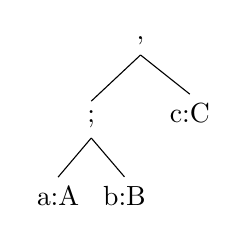
\begin{tikzpicture}
\Tree
[.,
    [.;
        [.a:A ]
        [.b:B ]
    ]
    [.c:C ]
    ]
\end{tikzpicture}

\caption{Bunches in \textbf{\em BI}}
\label{fig:bunches-bi}
\end{figure}

\begin{figure}[h]
  \begin{framed}
    \begin{flalign*}
      \text{Term Variables}\ \ \  x, y, z  &\in \text{Var} \nonumber\\
      \text{Patterns}\ \ \        p        &::= x \mid C \vec{x}\nonumber\\
      \text{Expressions}\ \ \     M, N     &::= x \mid \lambda^{*}x. M \mid \lambda^{\alpha}x. M \mid M N\nonumber\\
                                           &\mid \Case{M}{\{\texttt{inl}\ M \mapsto N ; \texttt{inr}\ M \mapsto N'\}}\mid \texttt{inl}\ M \mid \texttt{inr}\ M \nonumber\\
                                           &\mid \Let{x}{M}{N} \mid \nonumber
    \end{flalign*}
  \end{framed}
  \caption{Language Syntax}
  \label{fig:quill-terms}
\end{figure}
% Describe the language here

% Describe terms and patterns
Our term language is similar to that of simply typed lambda calculus involving variables and application
but we have 2 different kind of lambdas. The alpha lambda ($\lambda^{\alpha} x. M$) denotes sharing
of the argument term with the expression $M$ and the separating lambda term ($\lambda^{*} x. M$) that implies
the argument term has a separating context with the expression $M$. We also have polymorphic $\texttt{let}$
expressions to be able to define functions with a limited scope. Due to the rules of $\alpha\lambda$-calculus
it is easy to see that $f: \tau \sepimp \tau'; x:\tau \nvdash f x:\tau'$. As $f$ needs an argument that does
not share any resources with its context.

\begin{figure}[h]
  \begin{framed}\centering
    \begin{minipage}{0.45\linewidth}
      \begin{prooftree}
        \AxiomC{$\pi \in P$}
        \UnaryInfC{$P => \pi$}
      \end{prooftree}
    \end{minipage}
    \begin{minipage}{0.45\linewidth}
      \begin{prooftree}
        \AxiomC{$\bigwedge_{\pi \in Q} P => \pi$}
        \UnaryInfC{$P => Q$}
      \end{prooftree}
    \end{minipage}

    \begin{minipage}{0.45\linewidth}
      \begin{prooftree}
        \AxiomC{$$}
        \UnaryInfC{$P => \Un{(\tau \sepimp \tau')}$}
      \end{prooftree}
    \end{minipage}
    \begin{minipage}{0.45\linewidth}
      \begin{prooftree}
        \AxiomC{$$}
        \UnaryInfC{$P => \Un{(\tau \rightarrow \tau')}$}
      \end{prooftree}
    \end{minipage}

    \begin{minipage}{0.450\linewidth}
      \begin{prooftree}
        \AxiomC{$\tau = \sepimp \vee \tau = \overset{!}{\sepimp}$}
        \UnaryInfC{$P => \SeFun{\tau}$}
      \end{prooftree}
    \end{minipage}
    \begin{minipage}{0.450\linewidth}
      \begin{prooftree}
        \AxiomC{$\tau = \rightarrow \vee \tau = \overset{!}{\rightarrow}$}
        \UnaryInfC{$P => \ShFun{\tau}$}
      \end{prooftree}
    \end{minipage}

    \begin{minipage}{0.450\linewidth}
      \begin{prooftree}
        \AxiomC{$P => \Un{\tau}$}
        \UnaryInfC{$P => \tau \geq (v \overset{!}{\sepimp} v')$}
      \end{prooftree}
    \end{minipage}
    \begin{minipage}{0.450\linewidth}
      \begin{prooftree}
        \AxiomC{$P => \Un{\tau}$}
        \UnaryInfC{$P => \tau \geq (v \overset{!}{\rightarrow} v')$}
      \end{prooftree}
    \end{minipage}

    \begin{minipage}{0.450\linewidth}
      \begin{prooftree}
        \AxiomC{$$}
        \UnaryInfC{$P => \tau \geq (v \sepimp v')$}
      \end{prooftree}
    \end{minipage}
    \begin{minipage}{0.450\linewidth}
      \begin{prooftree}
        \AxiomC{$$}
        \UnaryInfC{$P => \tau \geq (v \rightarrow v')$}
      \end{prooftree}
    \end{minipage}

    \begin{minipage}{0.450\linewidth}
      \begin{prooftree}
        \AxiomC{$P => \tau \geq \phi t$}
        \AxiomC{$t\ \text{fresh}$}
        \BinaryInfC{$P => \tau \geq \phi$}
      \end{prooftree}
    \end{minipage}
    \begin{minipage}{0.450\linewidth}
      \begin{prooftree}
        \AxiomC{$P => \tau t \geq \phi$}
        \AxiomC{$t\ \text{fresh}$}
        \BinaryInfC{$P => \tau \geq \phi$}
      \end{prooftree}
    \end{minipage}

  \end{framed}
  \caption{Entailment Rules}
  \label{fig:entailment-rules}
\end{figure}


% The type constructors are added in order to allow programmers to define their own data types. They can be used to define sum and product types.
% \texttt{case} expression can be used to pattern match on the expression to express it in terms
% of individual sum types. Patterns are either term variables or constructor terms.


\section{Conventions and Notations}
The type assignment $\Gamma$ is a finite multiset of pairs of terms and types such that if two term variables occur
more than once, all of them must have same type. i.e. if $x:\sigma \in \Gamma$ and $x:\sigma' \in \Gamma$ then $\sigma \equiv \sigma'$.
The expression $P \mid \Gamma \vdash M : \sigma$ denotes the assersion that the term $M$ is of type $\sigma$
when the predicates in $P$ are satisfied and the free type variables in $M$ are specifed in type assigment $\Gamma$.
$\Gamma_{x}$ denotes the type assigment excluding the type variable $x$. $TV(\Gamma)$ denotes free type
variables in the environment $\Gamma$. $\Gamma \odot \Delta$ means that the contexts can either
be sharing union ($\Gamma \varoplus \Delta$) or separating union ($\Gamma \circledast \Delta$).

We try to emulate the behaviour of bunches using multisets and denote multiset union using $\Gamma \sqcup \Gamma'$.
The type assignment will be a collection of variables with an added annotation of sharing. If a resource $x$ is in
sharing with one or many resources $\bar{y}$ we would represent it as $x^{\bar{y}}:\tau$.
Further $\Gamma, x^{\bar{y}}:\tau$ would mean $\Gamma \sqcup \{x^{\bar{y}}:\tau\}$. We define a few auxilary functions on the
type assigments. Vars($\Gamma$) is the set of all the term variables in $\Gamma$. Shared($\Gamma$) computes
the set of all the term variables that are in sharing with each other. Used($\Gamma$) computes the
union of all the term variables in the type assignment and the term variables shared by each of those.
We define two partial operators on type assigments as shown in \cref{fig:context-operation}.
Two type assigments are said to be in disjoint union ($\circledast$) if they have no common used term.
If the type assignments have an exact overlapping of terms being used, it is said to be in a sharing union ($\varoplus$).
\begin{figure}[h]
  \begin{framed}
    \noindent
    \begin{flalign*}
      \text{Vars}(\Gamma, x^{\bar{y}}) &= \text{Vars}(\Gamma) \cup \{ x \}\\
      \text{Shared}(\Gamma, x^{\bar{y}}) &= \text{Shared}(\Gamma) \cup \{ \bar{y} \}\\
      \text{Used}(\Gamma) &= \text{Vars}(\Gamma) \cup \text{Shared}(\Gamma)\\
      (\Gamma, x^{\bar{y}})^{[a \mapsto \bar{b}]} &= \begin{cases}
        x \notin \bar{y}\ \ \ \ (\Gamma^{[a \mapsto \bar{b}]}, x^{\bar{y}}:\tau)\\
        x \in \bar{y}\ \ \ \  (\Gamma^{[a \mapsto \bar{b}]}, x^{(\bar{y}\backslash a)\cup\bar{b}}:\tau)
      \end{cases}\\
      \Gamma^{[\bar{a} \mapsto \bar{b}]} &= (\dots((\Gamma^{[a_1 \mapsto \bar{b}]})^{[a_2 \mapsto \bar{b}]})^{\dots})^{[a_2 \mapsto \bar{b}]}
    \end{flalign*}
  \end{framed}
  \caption{Auxilary Functions on Multisets}
  \label{fig:multiset-aux-function}
\end{figure}
\begin{figure}[h]
  \begin{framed}
    \begin{flalign*}
      \Gamma \circledast \Gamma' &= \Gamma \sqcup \Gamma' => \text{if}\ \text{Vars}(\Gamma) \# \text{Used}(\Gamma')\ \text{and}\ \text{Vars}(\Gamma')\# \text{Used}(\Gamma) \\
      \Gamma \varoplus \Gamma'   &= \Gamma \sqcup \Gamma' => \text{if}\ \text{Used}(\Gamma) \equiv \text{Used}(\Gamma')
    \end{flalign*}
  \end{framed}
  \caption{Context Operations}
  \label{fig:context-operation}
\end{figure}

\section{Typing Rules}
% Structural Rules
% Connective Rules
% forall, => Qualified type rules
% Entailment rules
We split our rules into multiple sections for legibility. The first section includes structrual rules
as shown in \cref{fig:structural-rules} and the second section includes connectives with introduction and elemination rules
as shown in \cref{fig:typing-rules}.

The tautology rule ([ID]) is a simple type assigment lookup for checking the type of the term.
The exchange rule ([EXCH]) justifies the fact that the order in which the type assignments are witnessed
in the multiset is insignificant and we can commute the individual term typing schemes within the multiset context
with no effect to the typing derivations. The contraction sharing rule [CTR-SH] and weakening sharing rule [WKN-SH]
says that we can duplicate or drop certain pairs of type assigments as per our convience as we know they are in sharing with other
terms that remain in the context. The contraction separation rule [CTR-UN] and weakening separation rule [WKN-SH] can be
applied to terms only if we can prove that they are of unrestricted type which is captured by introducting
the ($\Delta$ \texttt{un}) predicate on the type that is dropped or duplicated.

\begin{figure}[h]
  \begin{framed}
    % var
    \begin{minipage}{.5\textwidth}
      \begin{prooftree}
        \AxiomC{} \RightLabel{[ID]}
        \UnaryInfC{$P \mid x^{\bar{y}} : \sigma \vdash x : \sigma $}
      \end{prooftree}
    \end{minipage}
    % EXCH
    \begin{minipage}{.5\textwidth}
      \begin{prooftree}
        \AxiomC{$\Gamma \odot \Delta \vdash M : \sigma$} \RightLabel{[EXCH]}
        \UnaryInfC{$P \mid \Delta \odot \Gamma \vdash M : \sigma $}
      \end{prooftree}
    \end{minipage}
        % CTR UN
    \begin{minipage}{.5\textwidth}
      \begin{prooftree}
        \AxiomC{$P \mid \Gamma \circledast \Delta \vdash M : \sigma$}
        \AxiomC{$P'\vdash \Delta\ \texttt{un}$} \RightLabel{[CTR-UN]}
        \BinaryInfC{$P \mid \Gamma \vdash M : \sigma$}
      \end{prooftree}
    \end{minipage}
    % WKN UN
    \begin{minipage}{.5\textwidth}
      \begin{prooftree}
        \AxiomC{$P \mid \Gamma \vdash M : \sigma$}
        \AxiomC{$P' \vdash \Delta\ \texttt{un}$} \RightLabel{[WKN-UN]}
        \BinaryInfC{$P \mid \Gamma \circledast \Delta \vdash M : \sigma$}
      \end{prooftree}
    \end{minipage}
    % CTR Sh
    \begin{minipage}{.5\textwidth}
      \begin{prooftree}
        \AxiomC{$P \mid \Gamma \varoplus \Delta \vdash M : \sigma$} \RightLabel{[CTR-SH]}
        \AxiomC{$P \mid \Gamma \vdash M : \sigma$} \RightLabel{[CTR-SH]}
        \BinaryInfC{$P \mid \Gamma \vdash M : \sigma$}
      \end{prooftree}
    \end{minipage}
    % WKN Sh
    \begin{minipage}{.5\textwidth}
      \begin{prooftree}
        \AxiomC{$P  \mid \Gamma \vdash M : \sigma$} \RightLabel{[WKN-SH]}
        \UnaryInfC{$P \mid \Gamma \varoplus \Delta \vdash M : \sigma$}
      \end{prooftree}
    \end{minipage}
   \end{framed}
    \caption{Structural Typing Rules}
    \label{fig:structural-rules}
  \end{figure}

  The connective rules explained here.


  \begin{figure}[h]
    \begin{framed}
    % let
    \begin{minipage}{1\textwidth}
      \begin{prooftree}
        \AxiomC{$P \mid \Gamma \vdash M : \sigma$}
        \AxiomC{$P' \mid \Gamma_{x} \odot x: \sigma \vdash N: \tau$} \RightLabel{[LET]}
        \BinaryInfC{$P \cup P' \mid \Gamma \vdash \Let{x}{M}{N}: \tau$}
      \end{prooftree}
    \end{minipage}
    % forall I
    \begin{minipage}{0.5\textwidth}
      \begin{prooftree}
        \AxiomC{$P \mid \Gamma \vdash M: \sigma$}
        \AxiomC{$t \notin TV(\Gamma) \cup TV(P)$}\RightLabel{$[\forall I]$}
        \BinaryInfC{$P \mid \Gamma \vdash M: \forall t. \sigma$}
      \end{prooftree}
    \end{minipage}
    % forall E
    \begin{minipage}{0.5\textwidth}
      \begin{prooftree}
        \AxiomC{$P \mid \Gamma \vdash M: \forall t.\sigma$}\RightLabel{$[\forall E]$}
        \UnaryInfC{$P \mid \Gamma \vdash M: [\tau \backslash t] \sigma $}
      \end{prooftree}
    \end{minipage}
    % => I
    \begin{minipage}{0.5\textwidth}
      \begin{prooftree}
        \AxiomC{$P, \pi \mid \Gamma \vdash M : \rho$} \RightLabel{$[=> I]$}
        \UnaryInfC{$P \mid \Gamma \vdash M : \pi \Rightarrow \rho$}
      \end{prooftree}
    \end{minipage}
    % => E
    \begin{minipage}{0.5\textwidth}
      \begin{prooftree}
        \AxiomC{$P \mid \Gamma \vdash M : \pi \Rightarrow \rho$}
        \AxiomC{$P \Rightarrow \pi$} \RightLabel{$[=> E]$}
        \BinaryInfC{$P \mid \Gamma \vdash M: \rho$}
      \end{prooftree}
    \end{minipage}
    % -&> I
    \begin{minipage}{1\textwidth}
      \begin{prooftree}
        \AxiomC{$P \mid \Gamma^{[\emptyset\mapsto \{x\}]},x^{\text{Vars}(\Gamma)}: \tau \vdash M : \tau'$}
        \AxiomC{$P \Rightarrow \texttt{ShFun}\ \phi$}
        \AxiomC{$P \vdash \Gamma \geq \phi$} \RightLabel{$[\rightarrow I]$}
        \TrinaryInfC{$P \mid \Gamma \vdash \lambda^{\alpha}x. M : \phi \tau \tau'$}
      \end{prooftree}
    \end{minipage}
    % -&> E
    \begin{minipage}{1\textwidth}
      \begin{prooftree}
        \AxiomC{$P \mid \Gamma \vdash M : \phi \tau \tau'$}
        \AxiomC{$P \mid \Delta \vdash N : \tau'$}
        \AxiomC{$P => \texttt{ShFun}\ \phi$}
        \AxiomC{$P \vdash \Gamma \geq \phi$} \RightLabel{$[\rightarrow E]$}
        \QuaternaryInfC{$P \mid \Gamma \varoplus \Delta \vdash M N : \tau'$}
      \end{prooftree}
    \end{minipage}
    % -*> I
    \begin{minipage}{1\textwidth}
      \begin{prooftree}
        \AxiomC{$P \mid \Gamma,x^{\emptyset}: \tau \vdash M : \tau'$}
        \AxiomC{$P => \texttt{SeFun}\ \phi$}
        \AxiomC{$ P \vdash \Gamma \geq \phi$} \RightLabel{$[\sepimp I]$}
        \TrinaryInfC{$P \mid \Gamma \vdash \lambda^{*}x. M : \phi \tau \tau'$}
      \end{prooftree}
    \end{minipage}
    % -*> E
    \begin{minipage}{1\textwidth}
      \begin{prooftree}
        \AxiomC{$P \mid \Gamma \vdash M : \phi \tau \tau'$}
        \AxiomC{$P \mid \Delta \vdash N : \tau$}
        \AxiomC{$P => \texttt{SeFun}\ \phi$}
        \AxiomC{$P \vdash \Gamma \geq \phi$} \RightLabel{$[\sepimp E]$}
        \QuaternaryInfC{$P \mid \Gamma \circledast \Delta \vdash M N : \tau'$}
      \end{prooftree}
    \end{minipage}
  \end{framed}
    \caption{Connective Typing Rules}
    \label{fig:typing-rules}
\end{figure}

\begin{figure}[h]
  \begin{framed}
  \begin{minipage}{0.5\linewidth}
    \begin{prooftree}
      \AxiomC{$P => \texttt{Un}\ \tau$}\RightLabel{[\texttt{Un}-$\tau$]}
      \UnaryInfC{$P \vdash \tau\ \texttt{un}$}
    \end{prooftree}
  \end{minipage}
  \begin{minipage}{0.5\linewidth}
    \begin{prooftree}
      \AxiomC{$P,\pi \vdash \rho\ \texttt{un}$}\RightLabel{[\texttt{Un}-$\rho$]}
      \UnaryInfC{$P \vdash \pi => \rho\ \texttt{un}$}
    \end{prooftree}
  \end{minipage}
  \begin{minipage}{0.5\linewidth}
    \begin{prooftree}
      \AxiomC{$P, \texttt{Un}\ t \vdash \sigma\ \texttt{Un}$}\RightLabel{[\texttt{Un}-$\sigma$]}
      \UnaryInfC{$P \vdash \forall t.\sigma\ \texttt{un}$}
    \end{prooftree}
  \end{minipage}
  \begin{minipage}{0.5\linewidth}
    \begin{prooftree}
      \AxiomC{$\bigwedge_{x:\sigma \in \Gamma}P \vdash \rho\ \texttt{un}$}\RightLabel{[\texttt{Un}-$\Gamma$]}
      \UnaryInfC{$P \vdash \Gamma\ \texttt{un}$}
    \end{prooftree}
  \end{minipage}

  \begin{minipage}{0.5\linewidth}
    \begin{prooftree}
      \AxiomC{$P => \tau \geq \phi$}\RightLabel{[$\geq$-$\tau$]}
      \UnaryInfC{$P \vdash \tau \geq \phi$}
    \end{prooftree}
  \end{minipage}
  \begin{minipage}{0.5\linewidth}
    \begin{prooftree}
      \AxiomC{$P,\pi \vdash \rho \geq \phi$}\RightLabel{[$\geq$-$\rho$]}
      \UnaryInfC{$P \vdash (\pi => \rho) \geq \phi$}
    \end{prooftree}
  \end{minipage}
  \begin{minipage}{0.5\linewidth}
    \begin{prooftree}
      \AxiomC{$P, \texttt{Un}\ t \vdash \sigma \geq \phi$}\RightLabel{[$\geq$-$\sigma$]}
      \UnaryInfC{$P \vdash (\forall t.\sigma) \geq \phi$}
    \end{prooftree}
  \end{minipage}
  \begin{minipage}{0.5\linewidth}
    \begin{prooftree}
      \AxiomC{$\bigwedge_{x:\sigma \in \Gamma}P \vdash \rho \geq \phi$}\RightLabel{[$\geq$-$\Gamma$]}
      \UnaryInfC{$P \vdash \Gamma \geq \phi$}
    \end{prooftree}
  \end{minipage}
\end{framed}
  \caption{Typing Rules for Base cases}
  \label{fig:bi-base-typing-rules}
\end{figure}

\TODO{Explain what does it mean for a type to be less that other type}

\section{Syntax Directed Typing rules}
The typing rules explained in the previous section are not syntax directed and will not be fit
to develop an algorithm to develop a type inference algorithm. In this section we
will define syntax directed typing rules that will simplify our system.

\TODO{We will also prove equivance between the typing rules and syntax directed typing rules of our system}

\section{Modified Algorithm $\M$}
The type inference algorithm is given in \cref{fig:algorithm-m}
$\Sigma$ keeps track of all the used variables
$S$ is the substitution that is generated by the algorithm to infer the type of the
term using the context $\Gamma$. $X$ are the predicates for the qualified types.

$\mathcal{U}$ is a modified Robinson's unification algorithm[\cite{robinson_machine-oriented_1965}].
It generates kind preserving substitutions to unify types. The algorithm fails, if no such substitution exists.
We write $C \overset{U}{\sim}_{\kappa} C'$ for assertion that $U$ is the unifier
of the constructor types $C$ and $C'$.

\begin{flalign*}
  \tau \sim \tau' => \exists S. S \tau = \tau'
\end{flalign*}
\begin{figure}[h]
  \begin{framed}
    \begin{minipage}{0.5\linewidth}
      \begin{flalign*}
        Leq(\phi, \Gamma)  = \bigcup_{(x:\tau) \in \Gamma} \{P \mid P \vdash \phi \leq \tau \}
      \end{flalign*}
    \end{minipage}
    \begin{minipage}{0.5\linewidth}
      \begin{flalign*}
        \texttt{Un}(\Gamma)  = \bigcup\{P \mid (y:\sigma) \in \Gamma, P \vdash \sigma\ \texttt{un} \}
      \end{flalign*}
    \end{minipage}
    \begin{minipage}{0.5\linewidth}
      \begin{flalign*}
        \texttt{Weaken}(x, \sigma, \Sigma)  = \begin{cases}
          P\ \ \ \ &\text{if}\ x \notin \Sigma, P \vdash \sigma\ \texttt{un}\\
          \emptyset\ \ \ &otherwise
        \end{cases}
      \end{flalign*}
    \end{minipage}
    \begin{minipage}{0.5\linewidth}
      \begin{flalign*}
        \texttt{GenI}(\Gamma, P &=> \tau)  = \forall (ftv(S P, \tau)).S P => \tau \nonumber\\
        \text{where}\ &S\ \text{improves}\ \texttt{ftv}(P) \backslash \texttt{ftv}(\Gamma, \tau)\ \text{in}\ P
      \end{flalign*}
    \end{minipage}
    \begin{minipage}{1\linewidth}
      \begin{flalign*}
        \mathcal{C}(P, \Gamma, \Sigma)  = \{ x_i, x_j \mid \Gamma(x_i:\tau_1;x_j:\tau_2) \}
      \end{flalign*}
    \end{minipage}
  \end{framed}
  % Un
  % Weaken
  % GenI
  % \mathcal{C}(\Gamma, \Sigma)
  \caption{Auxilary definitions}
  \label{fig:aux-defs}
\end{figure}

\begin{figure}[h]
  \begin{framed}
    \begin{minipage}[ht]{1\linewidth}
      \centering
      \fbox{
        $\M(S, X;\Gamma \vdash M : \tau) = P, S', \Sigma$
      }
    \end{minipage}

    % x var
    \begin{minipage}{1\linewidth}
      \begin{flalign*}
        \M(S, X;\Gamma \vdash x : \tau) &= ([\vec{u} / \vec{t}]P), S' \circ S, \{x\} \nonumber \\
        \text{where}\ (x : \forall \vec{t}. P => \nu) &\in S \Gamma \nonumber\\
        S' &= \Unf([\vec{u} / \vec{t}]\nu, S \tau)
      \end{flalign*}
    \end{minipage}

    % \*x. M: t
    \begin{minipage}{1\linewidth}
      \begin{flalign*}
        \M(S, X;\Gamma \vdash \lambda ^{*} x. M : \tau) &= (P \cup Q), S', \Sigma \backslash x \nonumber \\
        \text{where}\ P; S'; \Sigma &= \M(\Unf(\tau, u_1 u_2 u_3) \circ S, X; \Gamma, x:u_2 \vdash M: u_3) \nonumber\\
        Q &= \{\SeFun{u_1}\} \cup \text{Leq}(u_1, \Gamma\mid_{\Sigma}) \cup \text{Weaken}(x, u_2, \Sigma)
      \end{flalign*}
    \end{minipage}

    % \&x. M: t
    \begin{minipage}{1\linewidth}
      \begin{flalign*}
        \M(S, X;\Gamma \vdash \lambda ^{\alpha} x. M : \tau) &= (P \cup Q), S', \Sigma \backslash x \nonumber \\
        \text{where}\ P; S'; \Sigma &= \M(\Unf(\tau, u_1 u_2 u_3) \circ S, X; \Gamma, x:u_2 \vdash M: u_3) \nonumber\\
        Q &= \{\ShFun{u_1}\} \cup \text{Leq}(u_1, \Gamma|_{\Sigma}) \cup \text{Weaken}(x, u_2, \Sigma)
      \end{flalign*}
    \end{minipage}

    % M N: t
    \begin{minipage}{1\linewidth}
      \begin{flalign*}
        \M(S, X;\Gamma \vdash M N : \tau) &= Q, R', \Sigma \cup \Sigma' \nonumber \\
        \text{where}\ P, R, \Sigma &= \M(S, X; \Gamma M:  u_1 u_2 \tau) \nonumber \\
        P', R', \Sigma' &= \M(R, X; \Gamma N: u_2) \nonumber\\
        \text{if}\ \mathcal{C}(\Gamma, \Sigma) &= \mathcal{C}(\Gamma, \Sigma') \nonumber\\
        \text{then}\ Q &= P \cup P' \cup \{\ShFun{u_1}\} \nonumber\\
        \text{else}\ Q &= P \cup P' \cup \{\SeFun{u_1}\} \cup \text{Un}(\Gamma|_{\Sigma \cap \Sigma'})
      \end{flalign*}
    \end{minipage}

    % let x = M in N: t
    \begin{minipage}{1\linewidth}
      \begin{flalign*}
        \M(S, X;\Gamma \vdash \Let{x}{M}{N} : \tau) &= (P \cup Q), R', \Sigma \cup \{\Sigma' \backslash x \} \nonumber\\
        \text{where}\ P, R, \Sigma &= \M(S, X;\Gamma \vdash M:u_1) \nonumber \\
        \sigma &= \text{GenI}(R\Gamma; R(P => u_1)) \nonumber\\
        P', R', \Sigma' &= \M(R, X;\Gamma, x:\sigma \vdash N : \tau) \nonumber\\
        Q &= \text{Un}(\Gamma|_{\Sigma \cap \Sigma'}) \cup \text{Weaken}(x, \sigma, \Sigma')
      \end{flalign*}
    \end{minipage}

    \begin{minipage}{1\linewidth}
      \begin{flalign*}
        \M(S, X;\Gamma \vdash \Case{M}{\{p_i \mapsto N_i\}_i}) &= (P_M \cup \{P_i\}), Q, \Sigma_M \cup \{\Sigma_i\} \nonumber\\
        \text{where}\ P_M, R_M, \Sigma_M &= \M(S, X;\Gamma \vdash M:u_1 \oplus u_2 \oplus \cdots \oplus u_n) \nonumber \\
        P_1, R_1, \Sigma_1 &= \M(R_M, X;\Gamma \vdash p_1:u_1 \vdash N_1: v) \nonumber \\
        P_i, R_i, \Sigma_i &= \M(R_{i-1}, X;\Gamma \vdash p_i:u_i \vdash N_i: v) \nonumber \\
        \Sigma' &= \bigcup_{i,j \leq n} (\Sigma_i \cap \Sigma_{j}) \nonumber\\
        Q &= \text{Un}(\Gamma|_{\Sigma'}) \cup \{\text{Weaken}(p_i, u_i, \Sigma_i)\}
      \end{flalign*}
    \end{minipage}
  \end{framed}
  \caption{Type Inference Algorithm $\mathcal{M}$}
  \label{fig:algorithm-m}
\end{figure}

\begin{figure}[h]
  \begin{framed}
    \begin{minipage}{1\linewidth}
      \begin{flalign*}
        \M(S, X;\Gamma \vdash C\ x) &= (P_M \cup \{P_i\}), Q, \Sigma_M \cup \{\Sigma_i\} \nonumber\\
        \text{where}\ C &= \forall \vec{t_1}. (\forall \vec{t_2}. \exists \vec{t_3}. Q => v') \sepimp v \nonumber\\
        P_M, R_M, \Sigma_M &= \M(S, X;\Gamma \vdash M:u_1 \oplus u_2 \oplus \cdots \oplus u_n) \nonumber \\
        P_1, R_1, \Sigma_1 &= \M(R_M, X;\Gamma \vdash p_1:u_1 \vdash N_1: v) \nonumber \\
        P_i, R_i, \Sigma_i &= \M(R_{i-1}, X;\Gamma \vdash p_i:u_i \vdash N_i: v) \nonumber \\
        \Sigma' &= \bigcup_{i,j \leq n} (\Sigma_i \cap \Sigma_{j}) \nonumber\\
        Q &= \text{Un}(\Gamma|_{\Sigma'}) \cup \{\text{Weaken}(p_i, u_i, \Sigma_i)\}
      \end{flalign*}
    \end{minipage}
  \end{framed}
  \caption{Type Inference Algorithm $\mathcal{M}$ (continued)}
  \label{fig:algorithm-m-cont}
\end{figure}

Here is how the naive recursive algorithm works

For Lambda
\begin{enumerate}
\item Get the bound variable
\item Assign a new type for bound variable
\item assign a new type variable for the body
\item Evaluate type of the body and assign it to the body type variable
\item return the type as (type of var) -> (type of body)
\end{enumerate}

Body can be made up of another lambda. In this case the same 5 steps will be triggered
or it is an application of 2 or more variables
In case of application 2 new type variable:
\begin{enumerate}
\item introduce type variables for left expression and right expression
  left expression a type $A \rightarrow B$ right expression gets the type $A$
\item recursively type check both of them
\item return the type of the complete application as $B$ if the type checking in previous step is successfully
\end{enumerate}


In Quill there are 2 kinds of lambdas:
\begin{enumerate}
\item Sharing Lambda $\lambda^{\alpha}$
\item Separating Lambda $\lambda^{*}$
\end{enumerate}
This helps us specify if the 2 variables are separated or have sharing
of resources between them.
The church encoding of a sharing pair will be represented as\\
$shPair = \lambda^{*} x \rightarrow \lambda^{\alpha} y \rightarrow \lambda^{*} sh \rightarrow sh\ x\ y$\\
This means that x and y may share resources
A separating pair is represented as\\
$sePair = \lambda^{*} x \rightarrow \lambda^{*}y \rightarrow \lambda^{*}se \rightarrow se\ x\ y$\\
This means that x and y do not share resources.
% By default we may assume that resources are always separating unless explicitly specified
% that they are sharing.

\section{Typing environment}

The typing environment in standard Milner-Damas algorithm
is a pair of identifier and its type.
We need to modify the typing environment so that it describes sharing.
% There can be many different ways of doing it.
In the current implementation we have
extended the typing environment to hold 2 more entities along with the
type of the identifier, a list of list of identifiers --- that describes the sharing of variables,
a scope tag---that identifies if the variable is global in the complete module or local to the definition.
Global variables can be used anywhere in the file or other code file if it is imported
All function names will be defaulted to global scope.
Local variables can be used only after they have been bound in the typing environment.
The new typing environment can be realized as:
\begin{minted}{haskell}
  type Env = Map Id (Type, [[Id]], Scope)
\end{minted}

% how is the list of list of ids help in identifying sharing

% how do you define a closure

% What do you mean by having a break in the closure

% The used field in the type-checker state

\section{Modification to Typechecking Algorithm}

To incorporate the sharing, we have to modify the typechecking algorithm.
The main reason to do that is to avoid adding $Un$ predicates to
shared variables that are not used. Take an example of $fst$ function
that returns the first argument of a shared pair
\begin{verbatim}
fst = \x -> \&y -> x
\end{verbatim}
In this case y should not be assigned an $Un$ predicate because
it is shared with x and x is indeed used.

The type checking algorithm has to be tweaked so that we keep track
of what all variables are shared and which ones are separate.

When we encounter an Alpha Lambda
\begin{enumerate}
\item Get the bound variable
\item Assign a new type for bound variable
\item Assign a new type variable for the body
\item add the variable in a sharing context
\item Evaluate type of the body and assign it to the body type variable
\item return the type as (type of var) -> (type of body)
\end{enumerate}


% The main problem is that we do not know when a sharing variable should be kept in scope
% or removed. In some cases we may need to keep it around for introducing the (>:=) predicates
% Some cases are 2 types:
% 1) The variable is used
% 2) The variable is not used

The type checking calls occur from left to right recursively.
While going down the recursion we keep on adding variables to the environment
We stop recursing at application. where we compute whether we have complete sharing to assign ShFun or SeFun.

While folding out of of the recursion we do 2 things:
1) keep track of the used variables (including implicitly used variables due to sharing)
2) generate new goals
a) depending on whether the the introduced variable was used
or its sharing member was used. Assign Un predicates and weaken if it is not used at all
b) introduce lesser-restricted predicates
3) Generate other new assumptions

We cannot determine when to get rid of the complete bunch.
\begin{verbatim}
\z -> \*x -> \&y -> y
\end{verbatim}
hence, when we are folding out of the final recursive but 1 call ie. for Lambda bound variable x

\section{Sharing}
What do we exactly mean by sharing?
There are 2 interpretations of sharing that i can think of
1) We have a resource $\mathcal{R}$, and 2 pointers $\alpha$, $\beta$. we say $alpha$, $\beta$ share if both of them point to the same resource $\mathcal{R}$
$\mathcal{R}$ is never exposed to the user space and can be manipulated only by using $\alpha$, $\beta$.
2) We have resource 


%%% Local Variables:
%%% mode: latex
%%% TeX-master: "../thesis-ku.tex"
%%% End:
        % Core syntax and Types with modified Algorithm M and unification
\chapter{Datatypes with resources}

We now see that we have two kinds of pairs. A sharing pair (\texttt{Pair$_{sh}$}) and a separating pair (\texttt{Pair$_{sep}$}) depending on
which arrow we use. The church encoding of both the pairs and their respective types are given in \ref{fig:bi-pairs-typing}.
Derivation proofs of both the pairs are given in \cref{sec:pairs}.
\begin{figure}
  \centering
  \begin{framed}
    \begin{flalign*}
      \text{Pair}_{sh} &: \tau \sepimp \tau' \rightarrow (\tau \sepimp \tau' \rightarrow \nu) \rightarrow \nu\\
      \text{Pair}_{sh} &= \lambda^{*} x. \lambda^{\alpha} by. \lambda^{\alpha} f. f x y\\
      \text{Pair}_{sep} &: \tau \sepimp \tau' \sepimp (\tau \sepimp \tau' \sepimp \nu) \sepimp \nu\\
      \text{Pair}_{sep} &= \lambda^{*} x. \lambda^{*} y. \lambda^{*} f. f x y
    \end{flalign*}
  \end{framed}
  \caption{Typing for Pairs in \textbf{\em BI}}
  \label{fig:bi-pairs-typing}
\end{figure}
We can now introduce 2 new type constructors in our type language $\otimes$ and $\with$
which represent separating pair and sharing pair respectively as shown in \cref{fig:pair-typing-rules}.
Simlar to products we have two flavors of sum types. multiplicative sum type ($\oplus$) when both the
types are separate and additive sum type ($\parr$) when both the types have sharing resources. Their
typing rules are shown in \cref{fig:bi-sum-types}. Proof derivation and definitions for
both the sum types are given in \cref{sec:sums}.

\begin{figure}[h]
  \begin{framed}
    \begin{minipage}{1\linewidth}
      \begin{prooftree}
        \AxiomC{$P \mid \Gamma  \vdash M : \tau$}
        \AxiomC{$P \mid \Delta \vdash N: \tau'$} \RightLabel{$[\with I]$}
        \BinaryInfC{$P \mid \Gamma \oplus \Delta \vdash \Pair{M;N} : \tau \with \tau'$}
      \end{prooftree}
    \end{minipage}
    \begin{minipage}{.5\linewidth}
      \begin{prooftree}
        \AxiomC{$P \mid \Gamma \vdash M: \tau \with \tau'$} \RightLabel{$[\with E_1]$}
        \UnaryInfC{$P \mid \Gamma \vdash \texttt{fst}_{sh}\ M: \tau$}
      \end{prooftree}
    \end{minipage}
    \begin{minipage}{.5\linewidth}
      \begin{prooftree}
        \AxiomC{$P \mid \Gamma \vdash M: \tau \with \tau'$} \RightLabel{$[\with E_2]$}
        \UnaryInfC{$P \mid \Gamma \vdash \texttt{snd}_{sh}\ M: \tau'$}
      \end{prooftree}
    \end{minipage}
    \begin{minipage}{1\linewidth}
      \begin{prooftree}
        \AxiomC{$P \mid \Gamma  \vdash M : \tau$}
        \AxiomC{$P \mid \Delta \vdash N: \tau'$} \RightLabel{$[\otimes I]$}
        \BinaryInfC{$P \mid \Gamma \circledast \Delta \vdash \Pair{M,N}: \tau \otimes \tau'$}
      \end{prooftree}
    \end{minipage}
    \begin{minipage}{.5\linewidth}
      \begin{prooftree}
        \AxiomC{$P \mid \Gamma \vdash M: \tau \otimes \tau'$} \RightLabel{$[\otimes E_1]$}
        \AxiomC{$P => \texttt{Un}\ \tau'$}
        \BinaryInfC{$P \mid \Gamma \vdash \texttt{fst}_{sep}\ M: \tau$}
      \end{prooftree}
    \end{minipage}
    \begin{minipage}{.5\linewidth}
      \begin{prooftree}
        \AxiomC{$P \mid \Gamma \vdash M: \tau \otimes \tau'$} \RightLabel{$[\otimes E_2]$}
        \AxiomC{$P => \texttt{Un}\ \tau$}
        \BinaryInfC{$P \mid \Gamma \vdash \texttt{snd}_{sep}\ M: \tau'$}
      \end{prooftree}
    \end{minipage}
  \end{framed}
  \caption{Derivable Typing rules for Pair types}
  \label{fig:pair-typing-rules}
\end{figure}

\begin{figure}[h]
\begin{framed}
\begin{minipage}[h]{0.5\linewidth}
  \begin{prooftree}
    \AxiomC{$\emptyset \mid \texttt{inl}_{sh}: \tau \sepimp \tau \parr \tau' \vdash x : \tau$}\RightLabel{[$\parr$I$_1$]}
    \UnaryInfC{$\emptyset \mid I \vdash \texttt{inl}_{sh}\ x: \tau \parr \tau'$}
  \end{prooftree}
\end{minipage}
\begin{minipage}[h]{0.5\linewidth}
  \begin{prooftree}
    \AxiomC{$\emptyset \mid \texttt{inr}_{sh}: \tau' \sepimp \tau \parr \tau' \vdash y : \tau'$}\RightLabel{[$\parr$I$_2$]}
    \UnaryInfC{$\emptyset \mid I \vdash \texttt{inr}_{sh}\ y: \tau \parr \tau'$}
  \end{prooftree}
\end{minipage}
\begin{minipage}[h]{1.0\linewidth}
  \begin{prooftree}
    \AxiomC{$\emptyset \mid \Gamma \vdash M : \tau \parr \tau'$}\RightLabel{[$\parr$E]}
    \AxiomC{$\emptyset \mid \Gamma \varoplus x:\tau \vdash N_1 : \nu$}
    \AxiomC{$\emptyset \mid \Gamma \varoplus y:\tau' \vdash N_2 : \nu$}
    \TrinaryInfC{$\emptyset \mid \Gamma \vdash \CaseSh{M}{\{ \texttt{inl}_{sh}\ x \mapsto N_1; \texttt{inr}_{sh}\ y \mapsto N_2\}}:\nu$}
  \end{prooftree}
\end{minipage}
% sum type I_l
\begin{minipage}{0.5\textwidth}
  \begin{prooftree}
    \AxiomC{$P \mid \Gamma \vdash M: \tau$}
    \UnaryInfC{$P \mid \Delta \vdash \texttt{inl}_{se}\ M: \tau \oplus \tau'$}
  \end{prooftree}
\end{minipage}
% sum type I_r
\begin{minipage}{0.5\textwidth}
  \begin{prooftree}
    \AxiomC{$P \mid \Gamma \vdash M: \tau_2$}
    \UnaryInfC{$P \mid \Delta \vdash \texttt{inr}_{se}\ M: \tau \oplus \tau'$}
  \end{prooftree}
\end{minipage}
% sum type E
\begin{minipage}{1\textwidth}
  \begin{prooftree}
    \AxiomC{$P \mid \Gamma \vdash M: \tau \oplus \tau'$}
    \AxiomC{$P \mid \Gamma \circledast x:\tau \vdash N :\nu$}
    \AxiomC{$P \mid \Gamma \circledast y:\tau' \vdash N':\nu$}\RightLabel{[$\oplus$E]}
    \TrinaryInfC{$P \mid \Gamma \vdash \CaseSe{M}{\{\texttt{inl}_{se}\ x \mapsto N; \texttt{inr}_{se}\ y \mapsto N'\}} : v $}
  \end{prooftree}
\end{minipage}
\end{framed}
\caption{Derivable Typing Rules for Sum Types}
\label{fig:bi-sum-types}
\end{figure}



\TODO{How do we write about type constructors?}

\begin{figure}[h]
  % sharing constructor
\begin{minipage}{1\textwidth}
  \begin{prooftree}
    \AxiomC{$P \mid \Gamma \vdash C: \tau_1 \sepimp \tau_2 \rightarrow \tau_3 \rightarrow \dots \rightarrow \tau_n \rightarrow T$}
    \AxiomC{$\Delta \equiv H(x_1 : \tau_1 ; x_2 : \tau_2 ; \ldots ; x_n:\tau_n)$}\RightLabel{$[\text{C-sh}]$}
    \BinaryInfC{$P \mid \Gamma; \Delta \vdash C \vec{x} : T $}
  \end{prooftree}
\end{minipage}
% Separating constructor
\begin{minipage}{1\textwidth}
  \begin{prooftree}
    \AxiomC{$P \mid \Gamma \vdash C: \tau_1 \sepimp \tau_2 \sepimp \tau_3 \sepimp \dots \sepimp \tau_n \sepimp T$}
    \AxiomC{$\Delta \equiv H(x_1: \tau_1, x_2:\tau_2, \dots ,x_n:\tau_n)$}\RightLabel{$[\text{C-se}]$}
    \BinaryInfC{$P \mid \Gamma, \Delta \vdash C \vec{x} : T $}
  \end{prooftree}
\end{minipage}

  \caption{User Defined Datatypes}
  \label{fig:ud-datatypes}
\end{figure}


The datatypes are user defined types:
There are 2 main kinds of non-recursive datatypes

1) data Choice a b = L a | R b

where the types a and b do not appear in both the constructors.
Choice here is a sum type a + b. How can we handle sum types in the current scenario?
1 way is to have a and b both not share resources. in this case we will have
a and b to be both un restricted.

a and b cannot direclty share resources. As the meaning of a sum type is that
either a or b can exist and not both. So we will always have separating arrow
for the sum types

Write the elemination rules for Either

for functions the closure has to be equal.

2) data Pair a b = P a b

The constructor uses both the resources a and b
Here we can have 2 subtypes:

a and b share resources or can be completely different.
We would want the programmer to specify whether the arguments are shared or separate.

For current purposes this syntactical specification is given via a modified syntax

data SeparatingPair a b = MkSeP a, b
data SharingPair a b = MkShP !! a b

We can of-course mix and match the sharing or separation.

data MixTuple a b c d e = MkMixTuple a,b;c,d

The question now that needs to be answered is how should the sharing be interpreted?
There are various options.

1. interpreted right to left. i.e. MkMixTuple (a, (b; (c,d)))
   so the b is shared with separating pair (c,d) and a is separate than b

2. interpreted left to right. i.e. MkMixTuple (((a, b);c),d)
   so the c is shared with separating pair (a,b) and d is separate from c

3. Sharing ; has precedence over separating , i.e. MkMixTuple a,(b;c),d

4. Separating , has lower precedence over ; i.e. MkMixTuple (a,b);(c,d)

This should be handled during the AST generating while parsing.
The type checking algorithm should be robust enough
to perform type checking either of these 4 types of sharing as they are
all perfectly valid scenarios.

Recursive datatypes have some kind of structural similarities within themselves

data Tree a = Leaf a | Node a (Tree a) (Tree a)

data Tree a b = Leaf b | Node a (Tree a b) (Tree a b)

Open questions:
How do we specify sharing of data between nodes?
eg. How can we say that all the leaves have shared data? and the data in nodes is sparating


What happens when lesser unrestrictedness with datatypes? Choice a b >:= f


\section{Examples}

\subsection{Pairs}

Our language has a notion of 2 kinds of pairs. The pairs representing resources that do not share
are denoted using separating pair $A \otimes B$. This means that when ever 



%%% Local Variables:
%%% mode: latex
%%% TeX-master: "../thesis-ku.tex"
%%% End:
      % sharing pair and weakening example Monad etc
\chapter{Conclusion and Future Work}

missing pieces here.
\global\long\def\bibname{References}

\bibliographystyle{apalike2}
\bibliography{Biblio/allcites}

\appendix
\chapter{Appendix}

\section{Proofs}

\subsection{Derivable Typing Rules For Product Types (Addiditive and Multiplicative Pairs)}
We start this section by adding few auxilary defitions for terms and types from first principles.

\begin{minipage}[h]{1.0\linewidth}
  \begin{prooftree}
    \AxiomC{$$}\RightLabel{[VAR]}
    \UnaryInfC{$\emptyset \mid y:B \vdash y: B $}\RightLabel{[VAR]}

    \AxiomC{$$}
    \UnaryInfC{$\emptyset \mid x: A \vdash x: A$}

    \AxiomC{$$}\RightLabel{[VAR]}
    \UnaryInfC{$\emptyset \mid f: A \sepimp B \rightarrow C \vdash f: A \sepimp B \rightarrow C $}\RightLabel{[$\sepimp E$]}
    \BinaryInfC{$\emptyset \mid x:A, f: A \sepimp B \rightarrow C \vdash f x: (B \rightarrow C)$}\RightLabel{[$\rightarrow E$]}

    \BinaryInfC{$\emptyset \mid y:B;x:A,f:A \sepimp B \rightarrow C \vdash f x y: C$}\RightLabel{[$EXCH$]}
    \UnaryInfC{$\emptyset \mid x:A;y:B,f:A \sepimp B \rightarrow C \vdash f x y: C$}\RightLabel{[$\sepimp I$]}
    \UnaryInfC{$\emptyset \mid x:A;y:B \vdash \lambda^{*}f. f x y: (A \sepimp B \rightarrow C) \rightarrow C$}\RightLabel{[$\rightarrow I$]}
    \UnaryInfC{$\emptyset \mid x:A \vdash \lambda^{\alpha}y. \lambda^{*}f. f x y: B \rightarrow (A \sepimp B \rightarrow C) \rightarrow C$}\RightLabel{[$\equiv$]}
    \UnaryInfC{$\emptyset \mid I, x:A \vdash \lambda^{\alpha}y. \lambda^{*}f. f x y: B \rightarrow (A \sepimp B \rightarrow C) \rightarrow C$}\RightLabel{[$\sepimp I$]}
    \UnaryInfC{$\emptyset \mid I \vdash \lambda^{*}x. \lambda^{\alpha}y. \lambda^{*}f. f x y: A \sepimp B \rightarrow (A \sepimp B \rightarrow C) \rightarrow C$}
  \end{prooftree}
\end{minipage}

We can now define sharing (additive) pair as:
\begin{framed}\centering
    $; = \lambda^{*}x. \lambda^{\alpha}y. \lambda^{*}f. f x y$
\end{framed}
and assign a new type to this pair and call it $\with$
\begin{framed}\centering
  $A \with B = (A \sepimp B \rightarrow C) \rightarrow C$
\end{framed}

\begin{minipage}[h]{1.0\linewidth}
  \begin{prooftree}
    \AxiomC{$$}\RightLabel{[VAR]}
    \UnaryInfC{$\emptyset \mid y:B \vdash y: B $}\RightLabel{[VAR]}

    \AxiomC{$$}
    \UnaryInfC{$\emptyset \mid x: A \vdash x: A$}

    \AxiomC{$$}\RightLabel{[VAR]}
    \UnaryInfC{$\emptyset \mid f: A \sepimp B \sepimp C \vdash f: A \sepimp B \sepimp C $}\RightLabel{[$\sepimp E$]}
    \BinaryInfC{$\emptyset \mid x:A, f: A \sepimp B \sepimp C \vdash f x: (B \sepimp C)$}\RightLabel{[$\sepimp E$]}

    \BinaryInfC{$\emptyset \mid y:B,x:A,f:A \sepimp B \sepimp C \vdash f x y: C$}\RightLabel{[$EXCH$]}
    \UnaryInfC{$\emptyset \mid x:A,y:B,f:A \sepimp B \sepimp C \vdash f x y: C$}\RightLabel{[$\sepimp I$]}
    \UnaryInfC{$\emptyset \mid x:A,y:B \vdash \lambda^{*}f. f x y: (A \sepimp B \sepimp C) \sepimp C$}\RightLabel{[$\sepimp I$]}
    \UnaryInfC{$\emptyset \mid x:A \vdash \lambda^{*}y. \lambda^{*}f. f x y: B \sepimp (A \sepimp B \sepimp C) \sepimp C$}\RightLabel{[$\equiv$]}
    \UnaryInfC{$\emptyset \mid I, x:A \vdash \lambda^{*}y. \lambda^{*}f. f x y: B \sepimp (A \sepimp B \sepimp C) \sepimp C$}\RightLabel{[$\sepimp I$]}
    \UnaryInfC{$\emptyset \mid I \vdash \lambda^{*}x. \lambda^{*}y. \lambda^{*}f. f x y: A \sepimp B \sepimp (A \sepimp B \sepimp C) \sepimp C$}
  \end{prooftree}
\end{minipage}
We can now define separating (multiplicative) pair as:
\begin{framed}\centering
    $,= \lambda^{*}x. \lambda^{*}y. \lambda^{*}f. f x y$
\end{framed}
We assign a new type to this pair construct and call it $\otimes$
\begin{framed}\centering
  $A \otimes B = (A \sepimp B \sepimp C) \sepimp C$
\end{framed}

We will abuse the notation of lambda calculus for $;$ and $,$ as use them as infix operators for syntactic convinence
\begin{flalign*}
  \langle x , y \rangle \equiv (,) x y\\
  \langle x ; y \rangle \equiv (;) x y
\end{flalign*}

We now define left and right projections or deconstructors for separating and sharing pairs below:

\begin{minipage}[h]{1.0\linewidth}
  \begin{prooftree}
    \AxiomC{$$}\RightLabel{[VAR]}
    \UnaryInfC{$\emptyset \mid x:A \vdash x: A $}\RightLabel{[WKN-SH]}
    \UnaryInfC{$\emptyset \mid x:A;y:B \vdash x: A $}\RightLabel{[$\rightarrow I$]}
    \UnaryInfC{$\emptyset \mid x:A \vdash \lambda^{\alpha}x : B \rightarrow A $}\RightLabel{[$\equiv$]}
    \UnaryInfC{$\emptyset \mid I, x:A \vdash \lambda^{\alpha}: B \rightarrow A $}\RightLabel{[$\sepimp I$]}
    \UnaryInfC{$\emptyset \mid I \vdash \lambda^{*}x. \lambda^{\alpha}y. x: A \sepimp B \rightarrow A$}
  \end{prooftree}
\end{minipage}

\begin{framed}
  \centering
    $\texttt{fst}_{sh} = \lambda^{*}x. \lambda^{\alpha}y. x$
\end{framed}
\begin{minipage}[h]{1.0\linewidth}
  \begin{prooftree}
    \AxiomC{$$}\RightLabel{[VAR]}
    \UnaryInfC{$\emptyset \mid y:B \vdash y: B $}\RightLabel{[WKN-SH]}
    \UnaryInfC{$\emptyset \mid x:A; y:B \vdash y: B $}\RightLabel{[$\rightarrow I$]}
    \UnaryInfC{$\emptyset \mid x:A \vdash \lambda^{\alpha}y : B \rightarrow B $}\RightLabel{[$\equiv$]}
    \UnaryInfC{$\emptyset \mid I, x:A \vdash \lambda^{\alpha}y: B \rightarrow B $}\RightLabel{[$\sepimp I$]}
    \UnaryInfC{$\emptyset \mid I \vdash \lambda^{*}x. \lambda^{\alpha}y. y: A \sepimp B \rightarrow B$}
  \end{prooftree}
\end{minipage}

\begin{framed}\centering
    $\texttt{snd}_{sh} = \lambda^{*}x. \lambda^{\alpha}y. y$
\end{framed}

\begin{minipage}[h]{1.0\linewidth}
  \begin{prooftree}
    \AxiomC{$$}\RightLabel{[VAR]}
    \UnaryInfC{$\Un{B} \mid x:A \vdash x:A $}

    \AxiomC{$$}
    \UnaryInfC{$\Un{B} => \Un{B}$}\RightLabel{[UN-$\Gamma$, UN-$\sigma$, UN-$\tau$]}
    \UnaryInfC{$\Un{B} \vdash y:B\ \texttt{un} $}\RightLabel{[WKN-UN]}

    \BinaryInfC{$\Un{B} \mid x:A, y:B \vdash x: A $}\RightLabel{[$\sepimp I$]}
    \UnaryInfC{$\Un{B} \mid x:A \vdash \lambda^{*}y. x : B \sepimp A $}\RightLabel{[$\equiv$]}
    \UnaryInfC{$\Un{B} \mid I, x:A \vdash \lambda^{*}y. x: B \sepimp A $}\RightLabel{[$\sepimp I$]}
    \UnaryInfC{$\Un{B} \mid I \vdash \lambda^{*}x. \lambda^{*}y. x: A \sepimp B \sepimp A$}
  \end{prooftree}
\end{minipage}

\begin{framed}\centering
    $\texttt{fst}_{sep} = \lambda^{*}x. \lambda^{*}y. x$
\end{framed}

\begin{minipage}[h]{1.0\linewidth}
  \begin{prooftree}
    \AxiomC{$$}\RightLabel{[VAR]}
    \UnaryInfC{$\Un{A} \mid y:B \vdash y: B $}

    \AxiomC{$$}
    \UnaryInfC{$\Un{A} => \Un{A}$}\RightLabel{[UN-$\Gamma$, UN-$\sigma$, UN-$\tau$]}
    \UnaryInfC{$\Un{A} \vdash x:A\ \texttt{un} $}\RightLabel{[WKN-UN]}

    \BinaryInfC{$\Un{A} \mid x:A, y:B \vdash y: B $}\RightLabel{[$\sepimp I$]}
    \UnaryInfC{$\Un{A} \mid x:A \vdash \lambda^{*}y.y: B \sepimp B $}\RightLabel{[$\equiv$]}
    \UnaryInfC{$\Un{A} \mid I, x:A \vdash \lambda^{*}y.y: B \sepimp B $}\RightLabel{[$\sepimp I$]}
    \UnaryInfC{$\Un{A} \mid I \vdash \lambda^{*}x. \lambda^{*}y. y: A \sepimp B \sepimp B$}
  \end{prooftree}
\end{minipage}

\begin{framed}\centering
    $\texttt{snd}_{sep} = \lambda^{*}x. \lambda^{*}y. y$
\end{framed}

We are now in a position to write the proof derivations for \cref{fig:derivable-typing-rules} using
the auxilary definitions from above.
\begin{framed}
  \noindent
  \begin{minipage}{0.5\linewidth}
    \begin{prooftree}
      \AxiomC{$\emptyset \mid I, M: A \with B \vdash \texttt{fst}_{sh}\ : A \sepimp B \rightarrow A$}\RightLabel{$\with E_1$}
      \UnaryInfC{$\emptyset \mid I \vdash \texttt{fst}_{sh}\  M : A$}
    \end{prooftree}
  \end{minipage}
  \begin{minipage}{0.5\linewidth}
    \begin{prooftree}
      \AxiomC{$\emptyset \mid I, M: A \with B \vdash \texttt{snd}_{sh}\ : A \sepimp B \rightarrow B$}\RightLabel{$\with E_2$}
      \UnaryInfC{$\emptyset \mid I \vdash \texttt{snd}_{sh}\  M : B$}
    \end{prooftree}
  \end{minipage}
  \noindent
  \begin{minipage}{1\linewidth}
    \begin{prooftree}
      \AxiomC{$P \mid \emptyset \vdash (;) : \with $}
      \AxiomC{$P \mid \Gamma  \vdash M : A$}
      \AxiomC{$P \mid \Delta \vdash N: B $} \RightLabel{$[\with I]$}
      \TrinaryInfC{$P \mid \Gamma;\Delta \vdash \langle M ; N \rangle: A \with B$}
    \end{prooftree}
  \end{minipage}
  \noindent
  \begin{minipage}{0.5\linewidth}
    \begin{prooftree}
      \AxiomC{$\Un{B} \mid I, M: A \otimes B \vdash \texttt{fst}_{sep}\ : A \sepimp B \sepimp A$}\RightLabel{$\otimes E_1$}
      \UnaryInfC{$\Un{B} \mid I \vdash \texttt{fst}_{sep}\  M : A$}
    \end{prooftree}
  \end{minipage}
  \begin{minipage}{0.5\linewidth}
    \begin{prooftree}
      \AxiomC{$\Un{A} \mid I, M: A \otimes B \vdash \texttt{snd}_{sep}\ : A \sepimp B \sepimp B$}\RightLabel{$\otimes E_2$}
      \UnaryInfC{$\Un{A} \mid I \vdash \texttt{snd}_{sep}\  M : B$}
    \end{prooftree}
  \end{minipage}
  \noindent
  \begin{minipage}{1\linewidth}
    \begin{prooftree}
      \AxiomC{$P \mid \emptyset \vdash (,) : \otimes $}
      \AxiomC{$P \mid \Gamma  \vdash M : A$}
      \AxiomC{$P \mid \Delta \vdash N: B $} \RightLabel{$[\otimes I]$}
      \TrinaryInfC{$P \mid \Gamma,\Delta \vdash \langle M , N \rangle: A \otimes B$}
    \end{prooftree}
  \end{minipage}
\end{framed}

\begin{landscape}
\subsection{Derivable Typing rules for Sum Types}
% choice
\noindent
  \begin{prooftree}
    \AxiomC{$$}
    \UnaryInfC{$\emptyset \mid  g:(B \sepimp E) \vdash g: (B \sepimp E)$}\RightLabel{[VAR]}

    \AxiomC{$$}
    \UnaryInfC{$\emptyset \mid f: (A \sepimp E) \vdash f: (A \sepimp E)$}\RightLabel{[VAR]}
    \AxiomC{$$}
    \UnaryInfC{$\emptyset \mid c: ((A \sepimp E) \sepimp (B \sepimp E) \sepimp E) \vdash c:((A \sepimp E) \sepimp (B \sepimp E) \sepimp E)$}\RightLabel{[VAR]}
    \BinaryInfC{$\emptyset \mid f:(A \sepimp E) \vdash c f: (B \sepimp E) \sepimp E$}\RightLabel{[$\sepimp$E]}

    \BinaryInfC{$\emptyset \mid  c:((A \sepimp E) \sepimp (B \sepimp E) \sepimp E), f:(A \sepimp E), g:(B \sepimp E) \vdash c f g : E$}\RightLabel{[$\sepimp$I]}
    \UnaryInfC{$\emptyset \mid  c:((A \sepimp E) \sepimp (B \sepimp E) \sepimp E), f:(A \sepimp E) \vdash  \lambda^{*} g. c f g :(B \sepimp E) \sepimp E$}\RightLabel{[$\sepimp$I]}
    \UnaryInfC{$\emptyset \mid  c:((A \sepimp E) \sepimp (B \sepimp E) \sepimp E) \vdash  \lambda^{*} f. \lambda^{*} g. c f g :(A \sepimp E) \sepimp (B \sepimp E) \sepimp E$}\RightLabel{[$\equiv$]}
    \UnaryInfC{$\emptyset \mid  I, c:((A \sepimp E) \sepimp (B \sepimp E) \sepimp E) \vdash  \lambda^{*} f. \lambda^{*} g. c f g :(A \sepimp E) \sepimp (B \sepimp E) \sepimp E$}\RightLabel{[$\sepimp$I]}\RightLabel{[$\sepimp$I]}
    \UnaryInfC{$\emptyset \mid I \vdash \lambda^{*} c. \lambda^{*} f. \lambda^{*} g. c f g : ((A \sepimp E) \sepimp (B \sepimp E) \sepimp E) \sepimp (A \sepimp E) \sepimp (B \sepimp E) \sepimp E$}
\end{prooftree}

% left
\noindent
\begin{prooftree}
  \AxiomC{$$}\RightLabel{[VAR]}
  \UnaryInfC{$\Un{A \sepimp E} \mid y: B  \vdash y : B$}

  \AxiomC{$$}\RightLabel{}
  \UnaryInfC{$\Un{A \sepimp E} \vdash \Un{A \sepimp E}$}\RightLabel{[WKN-UN]}
  \BinaryInfC{$\Un{A \sepimp E} \mid f: (A \sepimp E), y: B  \vdash y : B$}

  \AxiomC{$$}\RightLabel{[VAR]}
  \UnaryInfC{$\Un{A \sepimp E} \mid g: (B \sepimp E) \vdash g: (B \sepimp E)$}\RightLabel{[$\sepimp$I]}

  \BinaryInfC{$\Un{A \sepimp E} \mid f: (A \sepimp E), y: B, g: (B \sepimp E) \vdash g y : E$}\RightLabel{[EXCH]}
  \UnaryInfC{$\Un{A \sepimp E} \mid y: B, f: (A \sepimp E), g: (B \sepimp E) \vdash g y : E$}\RightLabel{[$\sepimp$I]}
  \UnaryInfC{$\Un{A \sepimp E} \mid y: B, f: (A \sepimp E) \vdash \lambda^{*} g. g y : (B \sepimp E) \sepimp E$}\RightLabel{[$\sepimp$I]}
  \UnaryInfC{$\Un{A \sepimp E} \mid y: B \vdash \lambda^{*} y. \lambda^{*} f. \lambda^{*} g. g y :(A \sepimp E) \sepimp (B \sepimp E) \sepimp E$}\RightLabel{[$\equiv$]}
  \UnaryInfC{$\Un{A \sepimp E} \mid  I, y: B \vdash \lambda^{*} y. \lambda^{*} f. \lambda^{*} g. g y :(A \sepimp E) \sepimp (B \sepimp E) \sepimp E$}\RightLabel{[$\sepimp$I]}\RightLabel{[$\sepimp$I]}
  \UnaryInfC{$\Un{A \sepimp E} \mid I \vdash \lambda^{*} y. \lambda^{*} f. \lambda^{*} g. g y: B \sepimp  (A \sepimp E) \sepimp (B \sepimp E) \sepimp E$}
\end{prooftree}

% right
\noindent
\begin{prooftree}
  \AxiomC{$$}\RightLabel{[VAR]}
  \UnaryInfC{$\Un{B \sepimp E} \mid x: A  \vdash x : B$}

  \AxiomC{$$}\RightLabel{}
  \UnaryInfC{$\Un{B \sepimp E} \vdash \Un{B \sepimp E}$}\RightLabel{[WKN-UN]}
  \BinaryInfC{$\Un{B \sepimp E} \mid g: (B \sepimp E), x: A  \vdash x : A$}

  \AxiomC{$$}\RightLabel{[VAR]}
  \UnaryInfC{$\Un{B \sepimp E} \mid f: (A \sepimp E) \vdash f: (A \sepimp E)$}\RightLabel{[$\sepimp$E]}

  \BinaryInfC{$\Un{B \sepimp E} \mid x: A, f: (A \sepimp E), g: (B \sepimp E) \vdash f x : E$}\RightLabel{[$\sepimp$I]}
  \UnaryInfC{$\Un{B \sepimp E} \mid x: A, f: (A \sepimp E) \vdash \lambda^{*} g. f x : (B \sepimp E) \sepimp E$}\RightLabel{[$\sepimp$I]}
  \UnaryInfC{$\Un{B \sepimp E} \mid x: A \vdash  \lambda^{*} f. \lambda^{*} g. f x :(A \sepimp E) \sepimp (B \sepimp E) \sepimp E$}\RightLabel{[$\equiv$]}
  \UnaryInfC{$\Un{B \sepimp E} \mid  I, x: A \vdash  \lambda^{*} f. \lambda^{*} g. f x :(A \sepimp E) \sepimp (B \sepimp E) \sepimp E$}\RightLabel{[$\sepimp$I]}\RightLabel{[$\sepimp$I]}
  \UnaryInfC{$\Un{B \sepimp E} \mid I \vdash \lambda^{*} x. \lambda^{*} f. \lambda^{*} g. f x: A \sepimp  (A \sepimp E) \sepimp (B \sepimp E) \sepimp E$}
\end{prooftree}


\end{landscape}

\subsection{Proofs for Soundness and Completeness}

\begin{theorem}
  Soundness of $\mathcal{M}$. If $\mathcal{M}(S, X; \Gamma \vdash M : \tau) = P, S', \Sigma$ then $S' P | S' (\Gamma\mid_{\Sigma}) \vdash M : S' \tau$
\end{theorem}

\begin{proof}
  Proof by induction on structure of $M$
  \begin{itemize}
  \item Case 1. $x$
  \item Case 2. $\lambda^{*} x. M$
  \item Case 3. $\lambda ^{\alpha}x. M$
  \item Case 4. $M\ N$
  \item Case 5. $\texttt{let}\ x = M\ \texttt{in}\ N$
  \end{itemize}

\end{proof}

\begin{theorem}
  Completeness of $\mathcal{M}$.
\end{theorem}
\begin{proof}
  Proof by induction on derivation on $M$
\end{proof}

\begin{theorem}
  $\mathcal{M}$ computes principal types.
\end{theorem}
\begin{proof}

\end{proof}
\end{document}

%%% Local Variables:
%%% mode: latex
%%% TeX-master: t
%%% End:
